\documentclass[english, 12pt, a4paper, sci, utf8, a-2b, online]{aaltothesis}
%\documentclass[english, 12pt, a4paper, sci, utf8, a-2b, print]{aaltothesis}
%\documentclass[english, 12pt, a4paper, sci, utf8, a-2b, print, twoside]{aaltothesis}

%% DO NOT MOVE OR REMOVE \setupthesisfonts
\setupthesisfonts

\usepackage{graphicx}

% Tables
\usepackage{tabularx,ragged2e}
\newcolumntype{C}{>{\Centering\arraybackslash}X} % centered "X" column
\usepackage{enumitem}
\usepackage{float}

% Code snippets
\usepackage{listings}
\usepackage{soul}

%% Feedback macros
\newcommand{\mycomment}[3]{\textcolor{#1}{#2:~#3}}
\newcommand{\jb}[1]{\noindent\mycomment{aaltoRed}{JB}{#1}}

% Code macros
\definecolor{codegreen}{rgb}{0,0.5,0}
\definecolor{codepurple}{rgb}{0.69,0,0.86}
\definecolor{codered}{rgb}{0.64,0.08,0.08}
\definecolor{codeteal}{rgb}{0,0.44,0.76}
\definecolor{codeyellow}{rgb}{0.48,0.37,0.15}
\definecolor{codedarklime}{rgb}{0.04,0.53,0.35}

\definecolor{darkred}{rgb}{0.5,0,0}
\definecolor{bgcolor}{rgb}{0.95,0.95,0.92}

\newcommand\YAMLcolonstyle{\color{black}\mdseries}
\newcommand\YAMLkeystyle{\color{darkred}\mdseries}
\newcommand\YAMLvaluestyle{\color{blue}\mdseries}

\makeatletter

% Here is a macro expanding to the name of the language
% (handy if you decide to change it further down the road)
\newcommand\language@yaml{yaml}

\expandafter\expandafter\expandafter\lstdefinelanguage
\expandafter{\language@yaml}
{
  % assuming a key comes first
  basicstyle=\YAMLkeystyle\ttfamily,
  sensitive=false,
  comment=[l]{\#},
  morecomment=[s]{/*}{*/},
  commentstyle=\color{codegreen},
  stringstyle=\YAMLvaluestyle,
  moredelim=[l][\color{orange}]{\&},
  moredelim=[l][\color{orange}]{*},
  % switch to value style at :
  moredelim=**[il][\YAMLcolonstyle{:}\YAMLvaluestyle]{:},
  literate =    {---}{{\ProcessThreeDashes}}3
                {>}{{\textcolor{codered}\textgreater}}1
                {|}{{\textcolor{codered}\textbar}}1
                {\ -\ }{{\mdseries\ -\ }}3,
}

% switch to key style at EOL
\lst@AddToHook{EveryLine}{\ifx\lst@language\language@yaml\YAMLkeystyle\fi}
\makeatother

\newcommand\ProcessThreeDashes{\llap{\color{black}\mdseries-{-}-}}

\lstdefinelanguage{javascript}{
  keywords={import, export, try, catch, return, throw, switch, case, if, while, do, else, break, await},
  ndkeywords={class, implements, typeof, function, this, new, true, false, null, boolean, const, var, in, async, =>},
  sensitive=false,
  comment=[l]{//},
  morecomment=[s]{/*}{*/},
  morestring=[b]',
  morestring=[b]",
  morestring=[b]`
}

\lstdefinelanguage{json}{
  basicstyle=\YAMLkeystyle, % assuming a key comes first
  sensitive=false,
  moredelim=[l][\color{orange}]{\&},
  moredelim=[l][\color{orange}]{*},
  moredelim=**[il][\YAMLcolonstyle{:}\YAMLvaluestyle]{:}, % switch to value style at :
  morestring=[b]',
  morestring=[b]",
  literate =    {---}{{\ProcessThreeDashes}}3
                {>}{{\textcolor{codered}\textgreater}}1
                {|}{{\textcolor{codered}\textbar}}1
                {\ -\ }{{\mdseries\ -\ }}3,
}

\lstdefinelanguage{Docker}{
  keywords={FROM, USER, ADD, RUN, COPY, WORKDIR, ENTRYPOINT, CMD},
  sensitive=false,
  comment=[l]{\#},
  morestring=[b]',
  morestring=[b]"
}

\lstdefinelanguage{bash}{
  keywords={if, while, do, else, done},
  ndkeywords={set, echo, cut, nsenter, docker, iptables},
  sensitive=false,
  comment=[l]{\#},
  morestring=[b]',
  morestring=[b]"
}

% https://github.com/julienc91/listings-golang/tree/master
\lstdefinelanguage{Golang}{
  morekeywords=[1]{package, import, func, type, struct, return, defer, panic, recover, select, var, const, iota},
  morekeywords=[2]{string,uint,uint8,uint16,uint32,uint64,int,int8,int16, int32, int64, bool, float32, float64, complex64, complex128, byte, rune, uintptr, error, interface},
  morekeywords=[3]{map, slice, make, new, nil, len, cap, copy, close, true, false, delete, append, real, imag, complex, chan},
  morekeywords=[4]{for, break, continue, range, go, goto, switch, case, fallthrough, if, else, default},
  morekeywords=[5]{Println, Printf, Error, Print,},
  sensitive=true,
  morecomment=[l]{//},
  morecomment=[s]{/*}{*/},
  morestring=[b]',
  morestring=[b]",
  morestring=[s]{`}{`},
}

\lstdefinestyle{mystyle}{
    backgroundcolor=\color{bgcolor},
    commentstyle=\color{codegreen},
    keywordstyle=\color{codepurple},
    ndkeywordstyle=\color{blue},
    numberstyle=\tiny\color{gray},
    stringstyle=\color{codered},
    basicstyle=\ttfamily,
    columns=flexible,
    breakatwhitespace=false,
    breaklines=true,
    captionpos=b,
    keepspaces=true,
    numbers=left,
    numbersep=5pt,
    showspaces=false,
    showstringspaces=false,
    showtabs=false,
    tabsize=2
}

\lstset{style=mystyle}

\usepackage{csquotes}
\usepackage{biblatex}
\addbibresource{./refs.bib}

% \usepackage{hyperref}
% \hypersetup{pdfpagemode=UseNone, pdfstartview=FitH,
%   colorlinks=true,urlcolor=red,linkcolor=blue,citecolor=black,
%   pdftitle={Default Title, Modify},pdfauthor={Your Name},
%   pdfkeywords={Modify keywords}}

%% For tables that span multiple pages; used to split a paraphrasing example in the appendix. If you don't need it, remove it.
\usepackage{longtable}

%% A package for generating Creative Commons copyright terms. If you don't use the CC copyright terms, remove it, since otherwise undesired information may be added to this document's metadata.
\usepackage[type={CC}, modifier={by-nc-sa}, version={4.0}]{doclicense}
%% Find below three examples for typesetting the CC license notice.

\degreeprogram{Computer, Communication and Information Sciences}
\major{Computer Science}
%\univdegree{BSc}
\univdegree{MSc}
%\univdegree{Lic}

\thesisauthor{Aarni Halinen}
\thesistitle{Security Risks for Sidecar Containers in Kubernetes}

\place{Espoo}
\date{29.12.2023}

\supervisor{Prof.\ Mario Di Francesco}
\advisor{M.Sc.\ (Tech.)\ José\ Luis\ Martin\ Navarro}
\advisor{M.Sc.\ (Tech.)\ Jacopo\ Bufalino}

%% If you do your thesis work in a company or another institute, give the name of the company or institution here. Otherwise, leave the macro empty, comment it out, or remove it. This will remove this field from the abstract page.
% \collaborativepartner{Company or institute name}

%% Aaltologo: syntax:
%% \uselogo{?|!|''}
%% The logo language is set to be the same as the thesis language.
%\uselogo{?}
%\uselogo{!}
\uselogo{''}

\copyrighttext{\noexpand\textcopyright\ \number\year. This work is licensed under a Creative Commons "Attribution-NonCommercial-ShareAlike 4.0 International" (BY-NC-SA 4.0) license.}{\noindent\textcopyright\ \number \year \ \doclicenseThis}
% \setboolean{writexmpdatafile}{false}

\begin{document}

\makecoverpage
\makecopyrightpage

\clearpage

%% Abstract texts
%% All the details (name, title, etc.) on the abstract page appear as specified above.

\keywords{Kubernetes, Container, Sidecar pattern, Network Security}

\begin{abstractpage}[english]
  The widespread adoption of containers has been a driving force behind the shift from monolithic applications to microservices.
  The modular nature of microservice architecture has allowed the development of distributed system design patterns such as the sidecar pattern, in which peripheral tasks are separated from the application containers as their own distinct containers.
  The sidecar pattern is often used to implement observability, log, and improve security with service meshes.

  This thesis examines the security risks associated with sidecar containers in Kubernetes container orchestration.
  It focuses on Kubernetes networking and Zero Trust security architecture to identify potential vulnerabilities that adversaries could exploit.
  The research reveals that Kubernetes only offers built-in security measures on a Pod-level, which can leave sidecar containers exposed to attack.

  The thesis introduces two proof-of-concept solutions aimed at establishing network isolation between application and sidecar containers.
  The first solution utilizes IPTables to enforce isolation, while the second employs Multus to mimic shared network namespace between containers in distinct Pods.

  Despite the demonstrated solutions for network isolation, the complexities of implementation and the need for specialized infrastructure pose challenges that may outweigh the benefits of such architectural modifications.
  Due to the challenges, the thesis explores the merits of sidecarless service mesh architectures such as Cilium and Istio Ambient Mesh, as an example of avoiding the risks with sidecars altogether.

  Ultimately, while the thesis presents viable proof-of-concept solutions for network isolation between application and sidecar containers, it advocates for a cautious approach, emphasizing the preference for established and well-tested components over custom-made implementations that need to be actively maintained.
\end{abstractpage}

%% Force a new page so that the possible Finnish or Swedish abstract does not begin on the same page
\newpage

\thesistitle{Sivuvaunukonttien turvallisuusriskit Kubernetes-orkestraatiossa}
\supervisor{Prof.\ Mario Di Francesco}
\advisor{DI José\ Luis\ Martin\ Navarro}
\advisor{DI Jacopo\ Bufalino}
% \degreeprogram{Elektroniikka ja sähkötekniikka}
% \major{Sopiva pääaine}
% \collaborativepartner{Yhtiön tai laitoksen nimi}
\date{29.12.2023}

\keywords{Kubernetes, konttiteknologia, sivuvaunumalli, verkkoturvallisuus}

\begin{abstractpage}[finnish]
  Konttiteknologian yleistyminen on ollut merkittävä tekijä siirryttäessä monoliittisista sovelluksista mikropalveluihin.
  Mikropalveluarkkitehtuurin modulaarisuus on mahdollistanut hajautettujen järjestelmäsuunnittelumallien, kuten sivuvaunumallin, kehittymisen.
  Sivuvaunumallissa sovelluksesta erilliset sivutehtävät kuten havainnointi, lokien kirjoittaminen tai palveluverkkojen välityspalvelimet voidaan toteuttaa omina erillisinä kontteinaan pääsovelluksen rinnalla.

  Tämä diplomityö tutkii turvallisuusriskejä, jotka liittyvät sivuvaunukontteihin Kubernetes-orkestraatiossa.
  Työ keskittyy Kuberneteksen verkkototeutukseen ja nollaluottamuksen tietoturva-arkkitehtuuriin ja tutkii sivuvaunukontteihin liittyviä tietoturvariskejä, joita hyökkääjät voisivat hyödyntää.
  Kubernetes tarjoaa valmiita tietoturvaominaisuuksia vain Pod-abstraktiotasolla, mikä altistaa sivuvaunukontteja hyökkäyksille.

  Työssä esotellään kaksi alustavaa ratkaisua, joiden avulla voidaan eristää sovellus- ja sivuvaunukonttien verkot toisistaan.
  Ensimmäinen ratkaisu perustuu IPTables-sääntöhin, kun taas toinen luo Multus-konttiverkkoliitännäisen avulla sivuvaunumallia imitoivan verkon kahden eristetyn kontin välille.

  Molemmat toteutukset ratkaisevat ongelman, mutta molempien monimutkaisuus ja tarve erikoistuneelle intrastruktuurille voi merkittävästi hankaloittaa ratkaisujen käyttöönottoa ja hyödyllisyyttä tuotantoympäristöissä.
  Kohdattujen haasteiden vuoksi työ tutkii myös sivuvaunuttomia palveluverkkoja, kuten Cilium ja Istio Ambient Mesh, keinona välttää sivuvaunuihin liittyvät turvallisuusriskit.

  Vaikka diplomityössä esitetäänkin ratkaisut sivuvaunukonttien verkkoeristykseen, on välttämätöntä korostaa vakiintuneiden ja hyvin testattujen komponenttien suosimista räätälöityjen ja aktiivista ylläpitoa vaativien toteutusten sijaan.
\end{abstractpage}

\newpage

\dothesispagenumbering{}

\mysection{Preface}

I want to thank my advisors, Jacopo Bufalino and José Luis Martin Navarro, for their valuable advice and guidance for this thesis.
I also want to thank my supervisor Mario Di Francesco for all his professional comments and support during the thesis process and earlier in my master's studies.

I also would like to thank all my friends, Radiodiodi and Sähköinsinöörikilta, for all the memorable moments during my (many) years of studies.
Last but not least, I want to thank my family for their support and encouragement during my studies and this thesis.

\vspace{5cm}
Helsinki, 29 December 2023 \\

\vspace{5mm}
{\hfill Aarni Halinen \hspace{1cm}}

\newpage

\thesistableofcontents

\mysection{Abbreviations}

\begin{tabular}{ll}
  API         & Application Programming Interface   \\
  BGP         & Border Gateway Protocol             \\
  BPF, cBPF   & (classic) Berkeley Packet Filter    \\
  cgroups     & Control groups                      \\
  CLI         & Command-line interface              \\
  CNCF        & Cloud Native Computing Foundation   \\
  CNI         & Container Network Interface         \\
  CRD         & Custom Resource Definition          \\
  DAC         & Discretionary Access Control        \\
  DoS         & Denial of Service                   \\
  eBPF        & Extended Berkeley Packet Filter     \\
  gRPC        & Google Remote Procedure Call        \\
  HTTP        & Hypertext Transfer Protocol         \\
  IPAM        & IP Address Management               \\
  IPC         & Inter-process communication         \\
  K8s         & Kubernetes                          \\
  LXC         & Linux Containers                    \\
  MAC         & Mandatory Access Control            \\
  mTLS        & Mutual Transport Layer Security     \\
  NAT         & Network Address Translation         \\
  NIC         & Network Interface Controller        \\
  OOM         & Out-of-memory                       \\
  OpenVZ      & Open Virtuozzo                      \\
  OS          & Operating System                    \\
  OSI         & Open Systems Interconnection        \\
  PID         & Process ID                          \\
  RCE         & Remote code execution               \\
  SELinux     & Security-Enhanced Linux             \\
  Seccomp     & Secure computing mode               \\
  TC          & Traffic Control                     \\
  VXLAN       & Virtual Extensible LAN              \\
  XDP         & eXpress Data Path                   \\
  ZTA         & Zero Trust Architecture             \\
\end{tabular}


\cleardoublepage

\thispagestyle{empty}

\section{Introduction} \label{sec:intro}

During the last decade, the IT industry has moved away from monolithic software applications and towards microservices.
The microservice architecture divides an application into a set of smaller, independent services that each handle a part of the business logic \cite{fowler2014microservices}.
Each service runs its own process, and the application data is sent between components using lightweight communication protocols such as the Hypertext Transfer Protocol (HTTP) and Google Remote Procedure Call (gRPC).
This approach increases software agility, as each service becomes an independent unit of development, deployment, operations, versioning, and scaling \cite{jamshidi2018microservices}.
This modularity is often associated with benefits such as faster delivery and better scalability.

The increasing use of containers has been a driving force behind the shift to microservices.
Containers are a lightweight virtualization technique where an application and all its dependencies are bundled into a single deployable unit running on the host machine kernel \cite{bui2015analysis}.
In a container-based microservice architecture, each service is bundled in its own container and deployed independently from the other services.
Popular container runtimes include \emph{Docker}, \emph{containerd}, and \emph{CRI-O}.

For more complex systems with multiple containers, scaling needs, and fault tolerance, a container orchestrator can be used.
Container orchestration tools automate the deployment, management, scaling, and networking of container workloads and handle tasks such as resource allocation and health monitoring.
The container orchestrators operate on top of a group of host machines, called a cluster, which serves as a resource pool for all container workloads.
Kubernetes is the most widely used orchestrator tool.

Similarly to how design patterns emerged from the birth of object-oriented software systems, the modularity of containers and microservices has allowed the development of distributed system design patterns \cite{burns2016design}.
The most common of these patterns is the sidecar pattern, in which peripheral tasks like logging and observability are split away as their own containers from the main application container.
The pattern allows easier installation of these nonfunctional features, while also keeping them away from the main container's source code.
Basically, the sidecar pattern is an extension of the modularity of the microservices architecture inside the microservice itself.
The benefits of the sidecar pattern are similar to microservices, allowing better resource allocation, re-use of components in other services, and providing a failure containment boundary, for example.
In Kubernetes, the basic unit of deployment is called a Pod, which may include one or more co-scheduled containers.
The Pod is analogous to a microservice, while it contains one main container and all its sidecars bundled into one deployable unit.

\subsection{Problem Statement}

Although the sidecar pattern makes it easier to add peripheral tasks to applications, it opens up questions about application security.
Quite often, developers rely on containers created by third parties for sidecar tasks.
The source code of these sidecar containers is not always available and finding vulnerabilities therein is not a trivial task.
Furthermore, malicious actors can use supply chain attacks and typo-squatting to trick victims into installing malicious sidecars to their clusters.
Once malicious attackers gain access to the sidecar, any misconfigurations or permissive security mechanisms put the whole cluster at risk.
Furthermore, Kubernetes is not secure by default; on a fresh installation, most of the included security mechanisms are in permissive settings or outright disabled.

Kubernetes offers limited security features at the container level.
Although containers have their own distinct security context definitions, all security-related policies and features are defined for Pods or Namespaces.
This means that sidecars, even if not required, inherit any capability and privileges from the main application.
Thus, any privileged workload, even in another container in the Pod, risks privilege escalation from the sidecar.
Additionally, Kubernetes' firewalling solution, NetworkPolicies, is applied to the entire Pod instead of individual containers.
This means that there are no built-in mechanisms in Kubernetes for protecting and isolating containers running in the same Pod from each other, which goes against the principle of least privilege.
Consequently, any exploitable security issue in a sidecar container could allow the attacker to move laterally to other containers in the Pod and escalate privileges.
This makes the sidecar an ideal starting point for attacks.

Zero trust architecture and the principle of least privilege are common security paradigms for limiting lateral movement and further escalation in a system if any component within has been compromised.
In both paradigms, the capabilities of an individual component are limited to only those that are required for the component to function.
The capabilities, such as network access and any container privileges, are explicitly given to the component that requires them, while everything else is denied.

If these paradigms are successfully applied to sidecars, sidecars could only use operations and network access required, while anything else would be blocked.
However, since Kubernetes provides limited security on the container-level, we need to find some other ways to implement these paradigms inside the Pods.
This thesis proposes a solution for restricting the capabilities of sidecars while minimally affecting the main container, thus improving security by extending the paradigms within the Pod.

\subsection{Thesis outline}

The following Chapter~\ref{sec:bg} gives background about containers and Kubernetes, and discusses about Kubernetes networking and container network interface plugins.
Chapter~\ref{sec:threats} analyzes security threats in a Kubernetes cluster with sidecars based on existing threat models and also demonstrates potential attack scenarios.
Chapter~\ref{sec:methods} defines the requirements of the solution and introduces the development environment used for the solutions.
Chapters~\ref{sec:pod-hardening} and \ref{sec:network-solution} propose solutions to mitigate security threats by hardening Pods and setting up network isolation, respectively.
Chapter~\ref{sec:solution} evaluates the pros and cons of the solutions.
Finally, Chapter~\ref{sec:discussion} discusses future research and concludes the thesis.

\clearpage

\section{Background} \label{sec:bg}

\subsection{Zero trust architecture}

Conventional network security has historically focused on perimeter defense \cite{kerman2020implementing}.
Subjects like workload resources and users inside the perimeter are often assumed to be trusted and implicitly given access inside the network, while any request originating outside the network is subject to more scrutiny.
Although the systems seem initially secure, the modern IT landscape with cloud-based systems, third-party components, remote workers, etc. increases the attack surface of threat actors.
Once any subject inside the perimeter is compromised, the attackers can gain access to all the resources that the subject is authorized to access and move laterally within the perimeter, escalating the attack on other resources.

Zero trust architecture (ZTA) is a security paradigm that focuses on data and resource protection and on the premise that trust must always be explicitly granted and continuously evaluated \cite{kerman2020implementing, rose2020zero}.
In contrast to a single perimeter defense, the focus in ZTA is to create fine-grained access rules around each of the resources while at the same time enforcing rules that deny other access, which is not explicitly allowed.
Following the principle of least privilege, the access rules are made as granular as possible so that the number of trusted subjects equals the actual number of subjects that require access.
This achieves a multi-layered security boundary, where the breach of one component through the most outward perimeter does not compromise the whole system.
Instead of having permission to access all resources within the perimeter, malicious actors could only laterally move to the resources that the compromised component required to function.
Any other component is still protected by its own perimeter, which would require another successful attack to be breached.
Thus, the compromised component is of limited usefulness to the attacker, instead of serving as a general attack vector against the system.

Zero-trust networking is based on the concept that the network, even if it is internal and behind a firewall, should never be trusted.
Instead of authenticating and authorizing only at the boundary, trust is verified at each component of the network.
This implies that each service should communicate securely in the network using protocols such as Mutual TLS (mTLS), and rely on more precise identifiers than just IP addresses.
Furthermore, access to a resource should be as limited as possible, and the policy can be further refined to restrict access based on, for example, HTTP routes on L7.
The ultimate aim in all cases is to achieve a policy of least privilege.

The complexity of managing the trust boundary in each component can be overwhelming.
Fortunately, Kubernetes can be extended with service meshes such as \emph{Istio}.
Service meshes provide a dedicated infrastructure layer in the application that allows the addition of features such as observability, traffic management, and security without having to modify the application code \cite{istio}.
Istio consists of two components: the data plane, which is composed of Envoy proxies that are deployed along with each service in the cluster, and the control plane.
The proxies intercept all network traffic of the parent service and implement features such as mTLS and traffic management, while also sending logs and other telemetry data to the control plane.
When the \lstinline{istio-injection=enabled} label is applied to a Namespace, any new Pods created in that Namespace will automatically have a sidecar injected into them.

\subsection{Containerization and Docker}

\begin{figure}[h!]
  \centering
  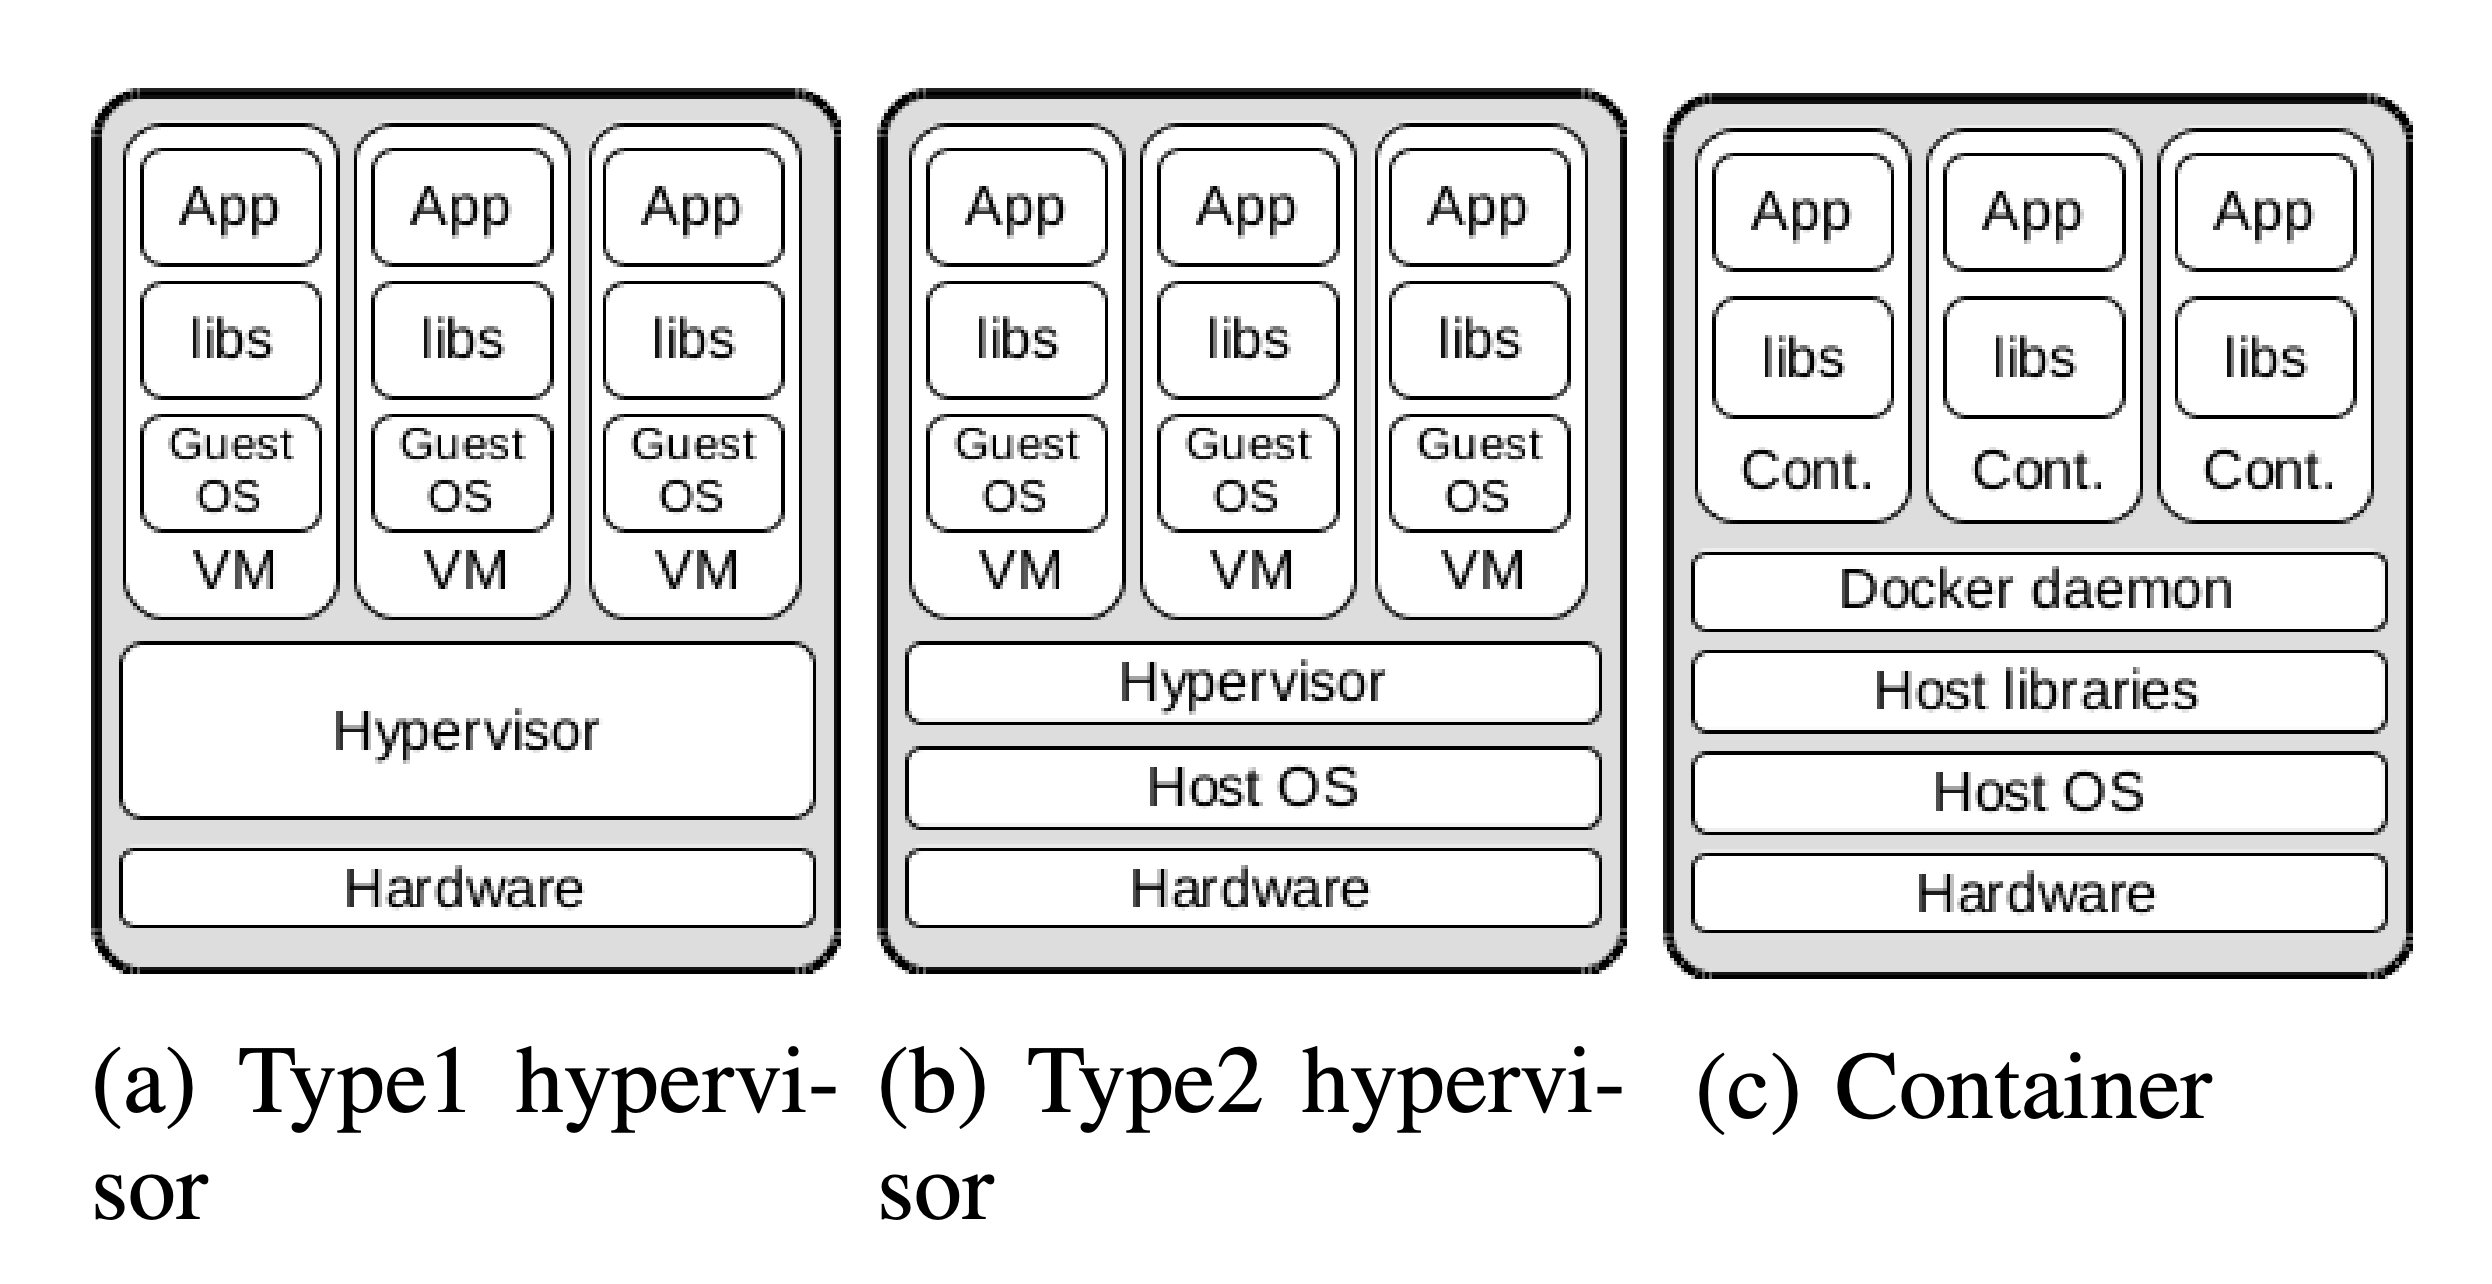
\includegraphics[width=\linewidth]{files/figure-1.png}
  \caption{Virtualization models \cite{combe2016docker}} % The image does not render nicely, would you be able to make one from scratch or find an SVG?
  \label{figure-1}
\end{figure}

Figure~\ref{figure-1} illustrates common virtualization models.
While traditional virtualization techniques virtualize workloads on top of a hypervisor that shares hardware resources between virtual machines, containerization is a technique where virtualization occurs at the operating system level \cite{merkel2014docker}.
Processes executing in containers run on the kernel of the host machine.
However, each container is isolated to its own network, process namespace, and so on; two containers on the same host OS do not know that they share resources.
Furthermore, containers are similarly isolated from accessing host OS resources.

BSD jails and \emph{chroot} can be considered early forms of containerization technology, so the idea of containers is not new \cite{combe2016docker}.
Recent Linux container solutions rely on two main implementations: Linux Containers (LXC) -based solution that relies on kernel features such as control groups (cgroups) and namespaces, and a custom kernel and Linux distribution called Open Virtuozzo (OpenVZ).
Docker \cite{docker} is a hugely popular LXC-based container runtime and provides an easy-to-use API and tooling for creating and managing containers.
Docker also provides containerization for other OSes as well.
However, in this thesis, we focus only on the Linux implementation.

\subsubsection{Linux containers}

The Linux containers technology implements container isolation and containment using a Linux kernel feature called namespaces \cite{lin2018measurement}.
Namespaces \cite{manpages-namespace} is a construct that wraps a global system resource in an abstraction that makes it appear to the processes in the namespace that they have their own isolated instance of the global resource.
There are a total of eight namespaces: i) \emph{Cgroup} which is used for resource management, ii) \emph{Inter-process communication} (IPC) which isolates POSIX message queues, etc., iii) \emph{Network} which isolates network devices, stack ports, etc., iv) \emph{Mount} for file system isolation, v) \emph{Process ID} (PID), vi) \emph{Time}, vii) \emph{User} for isolating user and group identifiers, and viii) \emph{UTS} which isolates hostnames and NIS domain names.
For example, the \emph{network} namespace provides each container with its own loopback device and even IPTables rules.
In another example, the \emph{mount} namespace ensures that the container has no visibility or access to the host's or other container's file system.
Compared to other namespaces that concern the isolation of kernel data, \emph{cgroups} focuses on limiting available system resources per namespace \cite{lin2018measurement}.
Each namespace can be configured with its own limits on CPU and memory usage and available devices.
Using Docker as an example, setting \lstinline{--cpu}, \lstinline{--memory} and \lstinline{--devices} options will limit available resources for the container.

Since all containers and the host machine run on the same kernel, any container that manages to break out from isolation may compromise other containers, the host, and the whole kernel.
To combat this container breakout, several security mechanisms are adopted from the Linux kernel to restrict the capabilities of containers \cite{lin2018measurement}.
These include Discretionary Access Control (DAC) mechanisms like Capability \cite{manpages-capabilities} and Secure computing mode (seccomp) \cite{manpages-seccomp}, and Mandatory Access Control (MAC) mechanisms such as Security-Enhanced Linux (SELinux) and AppArmor \cite{apparmor}.
With Capability, the superuser (i.e., the root user) privilege is divided into distinct units, each of which represents permission to process some specific kernel resources.
The feature turns the binary "root/non-root" security mechanism into a fine-grained access control system, which makes it easier to follow the principle of least privilege.
For example, processes like web servers that simply need to bind on an Internet domain privileged port (numbers below 1024) do not need to run as root; they can be granted with \lstinline{CAP_NET_BIND_SERVICE} capability instead \cite{docker-security}.
The Seccomp mechanism constrains the system calls that a process can invoke.
The available system calls are defined for a container through the Seccomp profile, which is defined as a JSON file.
The default Docker Seccomp profile \cite{docker-default-seccomp} includes more than 300 system calls.
SELinux is integrated into CentOS/RHEL/Fedora distributions and utilizes a label-based enforcement model, while AppArmor is available in Debian and Ubuntu distros and adopts a path-based enforcement model \cite{lin2018measurement}.

\subsubsection{Docker}

\begin{figure}[h!]
  \centering
  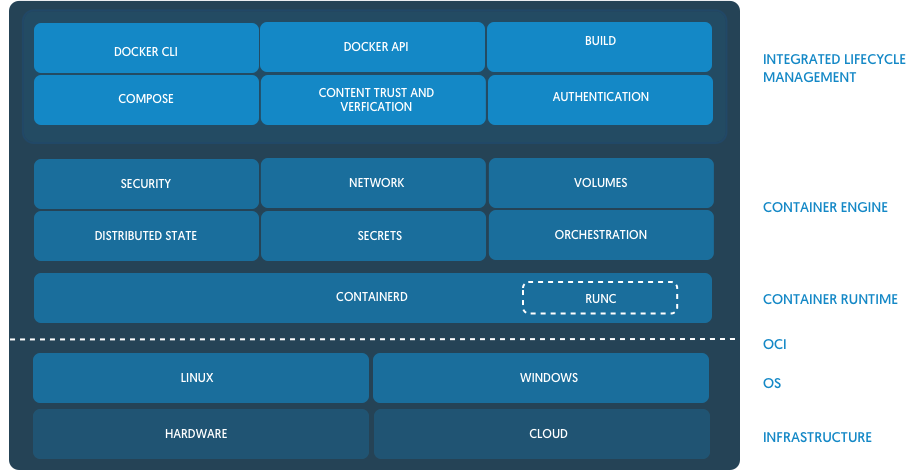
\includegraphics[width=\linewidth]{files/docker-arch.jpeg}
  \caption{Docker architecture \cite{containerd}}
  \label{figure-docker}
\end{figure}

Docker is an open-source container technology written in Go and launched in 2013 \cite{docker-what}.
The platform consists of the Docker Engine, a container runtime and packaging tool, and Docker image registries such as the Docker Hub public image repository and the Docker desktop application \cite{docker-overview}.
The engine functions as a client-server RESTful HTTP API application, with the Docker daemon acting as a server, managing and executing all the containers.
As illustrated in Figure~\ref*{figure-docker}, the daemon serves as a high-level container runtime and uses \emph{runC} and \emph{containerd} to create and run the containers in a system.

The Docker client is a command-line tool that provides a user interface to command the daemon, and thus containers.
By exposing the API outside the host machine, the architecture enables remote control of the daemon with the client.
Remote communication with the API should be carried out over TLS for security reasons.

Docker image is a read-only template with instructions for creating a Docker container \cite{docker-overview}.
Images are often based on another image, such as OS images \textbf{ubuntu} and \textbf{alpine}, with some additional customizations, such as the installation of web server binaries.
Customizations are added to the image as a series of data layers so that each new command creates a new layer.
This process makes image distribution more efficient since only the changes between layers must be distributed \cite{bui2015analysis}.
Layering is achieved with a special file system inspired by UnionFS that allows files and directories in different file systems to be combined into a single consistent file system.

Docker users can share their custom images publicly or privately in Docker Hub, or even host their own image registry platform.
Most cloud providers also offer container registry services, so even proprietary software can be published in a private registry and used by other cloud services, like Kubernetes clusters.
Whenever the image is not found locally, the client automatically attempts to search and pull the image from the connected registries.

\subsection{Kubernetes}

While container runtimes are used to create and destroy containers, container orchestrators are used as a system to automate the deployment, scaling, and management of containerized applications.
Kubernetes (K8s) \cite{kubernetes} is an open-source container orchestrator released in 2014.
It is hosted by the Cloud Native Computing Foundation (CNCF), but its roots are at Google, where it was developed as an alternative to Google's proprietary Borg and Omega orchestrators \cite{burns2016borg}.
A Kubernetes cluster consists of a set of servers, called Nodes, on which application containers are scheduled by the system.
This automation provides resilience and efficient resource utilization for workloads in the cluster: if a container or Node fails, the system attempts to restart and reschedule containers to maintain the desired cluster state.

\subsubsection{Kubernetes objects}

\textbf{Pods} are the basic atomic scheduling unit in Kubernetes.
Pods consist of one or more tightly coupled containers with shared storage volume and networking \cite{k8s-docs-pods}.
Containers in a Pod are always co-located and co-scheduled and run in a shared context, i.e. a set of Linux namespaces.
Network, UTS, and IPC namespaces are shared by default, and the process namespace can be shared with \lstinline{v1.PodSpec.shareProcessNamespace}.
The common network namespace means that containers in a Pod can communicate with each other via localhost, have a common IP address, and cannot reuse the same port numbers.
In addition to the normal application container, Pods can include special \lstinline{initContainers} that are run only on Pod startup.
These Pods are used to modify the Pod context before the actual workload starts.
Multiple \lstinline{initContainers} are run sequentially, and a failing container blocks the execution of the following initialization and normal workloads.

If a Pod fails, a replacement Pod is not automatically created.
Quite often, developers want to have more control over the compute resources and specify a target state for them.
This includes replication, scaling, and distribution among various nodes.
To meet these needs, Kubernetes provides additional resources.

Instead of directly creating Pods, \textbf{Deployment} workload resources can be used to create Pods in a cluster \cite{k8s-docs-pods}.
With Deployments, the user describes the desired state in a declarative manner.
The Kubernetes control loop then creates \textbf{ReplicaSet} based on the Deployment resource, which in turn guarantees the availability of the desired number of Pods \cite{k8s-docs-deployment}.
\textbf{DaemonSet} on the other hand is a workload resource that ensures that all or some Nodes run a copy of a Pod.
Typical use cases for daemons are running Node monitoring and logging, and network plugins, which are discussed in depth in Chapter~\ref{cni}.

All Pods in the cluster share the same subnet and can access each other via IP address.
However, connecting to a Pod with an IP address is suboptimal, since Pods are ephemeral.
A dead Pod, even if controlled by a ReplicaSet, is not guaranteed to receive the same IP address on restart.
Additionally, each replica in a horizontally scaled system has its own IP address.
This leads to the following problem: how do the clients using the system find and keep track of the IP addresses used by the workload? The \textbf{Service} abstraction solves the problem.

\textbf{Services} are an object for exposing groups of Pods over a network \cite{k8s-docs-services}.
The object defines a set of endpoints, that is, the targeted Pods, along with a policy about how to make the Pods accessible.
The targeted Pods are determined with a \lstinline{selector} field in the object specification.
Meanwhile, the \lstinline{type} field determines how the Service is exposed.
There are four different \textbf{ServiceTypes}: i) the default \textbf{ClusterIP} which exposes the Service inside the cluster with its own IP address, ii) \textbf{NodePort} which exposes the service in each Node's IP address on static port (by default within a range of 30000-32767), iii) \textbf{LoadBalancer} which exposes the Service externally using cloud provider's load balancer, and iv) \textbf{ExternalName} which is used to map Service to DNS name instead of a group of Pods.
The field is designed as a nested functionality; each \textbf{ServiceType} level adds up to the previous one.

% \jb{Usually services are proxies that route requests to the different Pods. There are also Headless services that only add DNS entries for the Pods.}

\textbf{Namespaces} allow logical grouping of resources under a single name.
New Kubernetes cluster starts with four namespaces: \emph{default}, \emph{kube-node-lease}, \emph{kube-public} and \emph{kube-system}.
Namespaced objects like Deployments, Services, and Pods are always deployed under a namespace which is \emph{default} if not explicitly defined.
\emph{kube-system} is the namespace for all objects created by the Kubernetes system, which is discussed in more detail in the next Chapter~\ref{control-plane}.
Namespaces also provide a scope for naming; names of resources must be unique within a namespace, but not across namespaces.
Namespaces are also used to enforce resource quotas, access control, and isolation for cluster users, for example, in multitenancy setups.
Pod Security Standards \cite{k8s-docs-pss}, which are used by the Pod Security admission controller, are also defined at the namespace level.
Admission controllers are discussed in Chapter~\ref{admission-controllers}.

\textbf{Custom Resource Definitions} (CRD) are used to define new resources that are not available in a default Kubernetes installation \cite{k8s-docs-crd}.
Once a custom resource is installed, users can create and access custom resource objects with \lstinline{kubectl}, similarly to any other built-in resource.
On their own, custom resources can only be used to store and retrieve structured data.
When combined with a custom controller, custom resources can be used to add new functionality to the cluster.
In Kubernetes, controllers are constructs that watch the current state of the cluster and keep track of the desired state.
If the states differ, the controller makes or requests changes so that the cluster state moves closer to the desired one.
Specifically, the controllers are implemented as \textbf{Operators} following the \emph{operator-pattern} \cite{k8s-docs-operators}.
The Operators are clients of the Kubernetes API that implement the control loop on a Custom Resource.
They are often deployed as Deployments and behave similarly to any other container workload in the cluster.

\subsubsection{Kubernetes components} \label{control-plane}

\begin{figure}[h!]
  \centering
  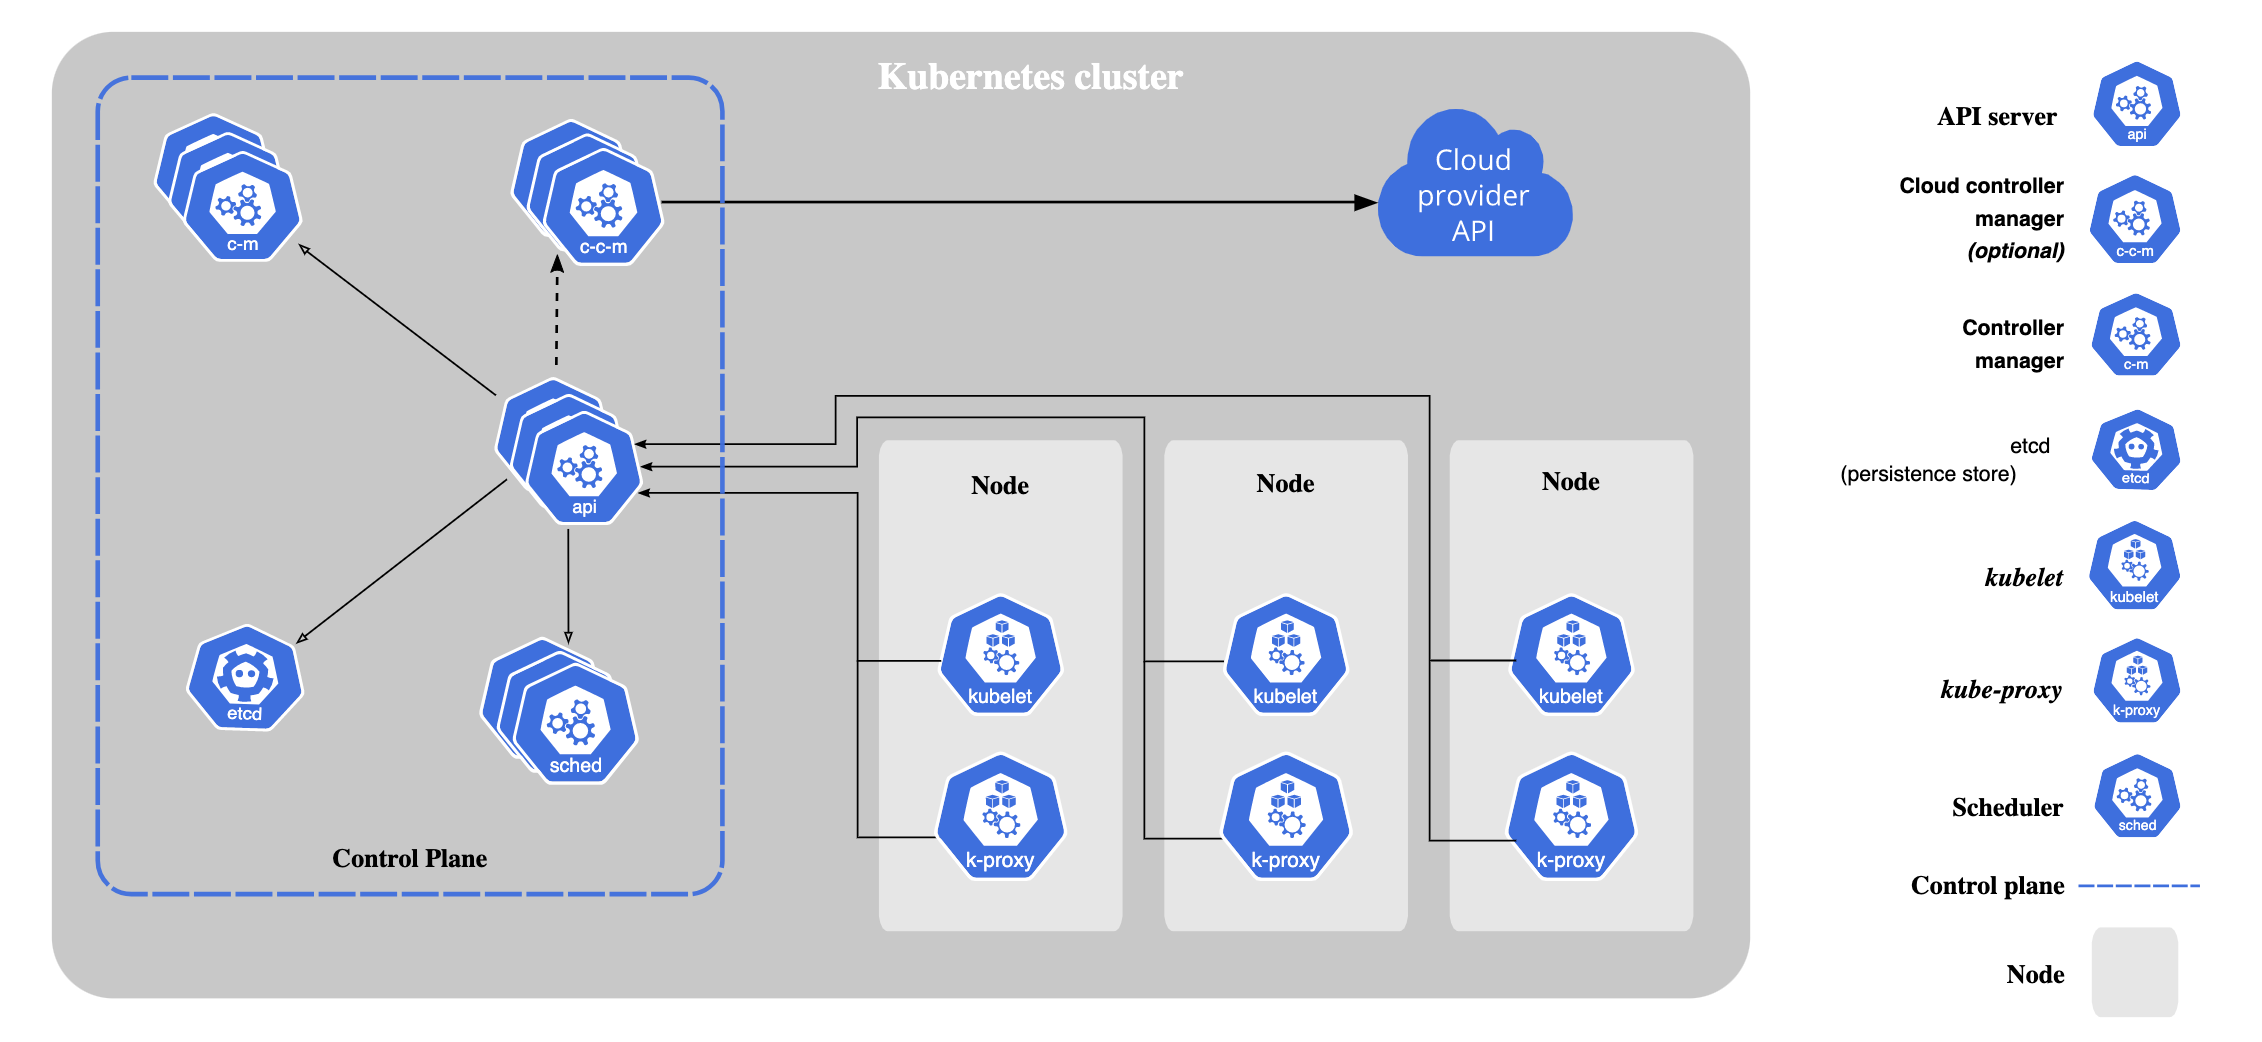
\includegraphics[width=\linewidth]{files/k8s-arch.png}
  \caption{Kubernetes cluster architecture \cite{k8s-docs-control-plane}}
  \label{figure-2}
\end{figure}

Figure~\ref{figure-2} describes the Kubernetes cluster with a control plane and three worker nodes.
The control plane consists of components that control, monitor, and store the state of the cluster; essentially, these are the components that are needed for the complete and working Kubernetes cluster \cite{k8s-docs-control-plane}.
The control plane components can run on any worker node.
However, clusters often have a specialized master node for control plane components, which does not run any other containers.
For fault tolerance and high availability, control plane components should run on multiple Nodes in production environments.
The control plane consists of these main components:

\textbf{API server} is a front-end component of the control plane.
It is an HTTP server that is used to send commands to the cluster.
The server handles the authentication and validation of the commands.
For valid commands, the server then forwards these to other control plane components that then modify the cluster state.
The easiest way to send commands to the server is by using the \lstinline{kubectl} command-line interface (CLI), which actively sends the commands as HTTP under the hood.
The main implementation of the server is \emph{kube-apiserver}.
The server can be horizontally scaled by running several instances on multiple Nodes and load-balancing traffic between the instances.

\textbf{Etcd} \cite{etcd} is a highly consistent, distributed key-value store.
It is the stateful component of the control plane: all of the cluster data is stored in etcd.
Thus, the stability of the component is critical for the whole cluster.
To tolerate failures, etcd implements a leader-based architecture.
Multiple etcd clients automatically elect a leader instance as the source of truth.
Other instances periodically update their state from the leader instance, so that the state stays eventually consistent across all instances.
On leader failure, the other instances automatically elect a new leader to keep the system functioning.

\textbf{Scheduler} watches for newly created Pods that have no assigned worker Node and selects one of the active Nodes for them to run on \cite{k8s-docs-control-plane}.
Scheduling takes into account resource availability on Nodes, Pod resource requirements, object specification affinity rules and hardware, software, and policy constraints, among others.

\textbf{Controller manager} is a control plane component that runs all the controller loop processes \cite{k8s-docs-control-plane}.
Controller loops, like the Deployment controller, continuously watch the current and desired cluster state.
When the states differ, they send commands via the API server so that the cluster moves toward the desired state.
All built-in controllers are compiled into a single binary, even though the controllers are logically different processes.

Each Node also has components that are essential for Kubernetes to work properly.
\textbf{Kubelet} is an agent that ensures that containers are running in a Pod \cite{k8s-docs-control-plane}.
It receives a set of Pod specifications from the API server and ensures that containers are running on the Node, follow the Pod specifications, and are healthy.
\textbf{Kubelet} only manages containers created by Kubernetes.
\textbf{Kube-proxy} maintains the network rules on Nodes.
Part of the Service objects' networking is implemented by \textbf{kube-proxy}; the proxy writes IPTables rules that route traffic \cite{cilium-proxy-free}.

\subsubsection{Admission controllers} \label{admission-controllers}

Admission controllers are a feature of the Kubernetes API server, used to validate and modify requests made to the server \cite{k8s-docs-admission}.
The controllers execute before the request is executed but after it is authenticated and authorized by the server.
Several important features of Kubernetes are implemented with admission controllers, and these should be enabled on a properly configured API server.
In addition to the built-in controllers, Kubernetes provides \textbf{MutatingAdmissionWebhook} and \textbf{ValidatingAdmissionWebhook} controllers for building its own admission logic.

Admission controllers can be validating, mutating, or both \cite{k8s-docs-admission}.
Mutating controllers may modify related objects to the requests they admit while validating controllers either approve or reject the request.
The control process first executes the mutating controllers so that no mutations occur after the validation.
If a controller in either phase rejects the request, the request is not processed further and the error is returned to the end-user.

One notable Admission controller is the \textbf{PodSecurity} controller.
The controller validates the Pods before they are admitted, making sure that the requested Pod security context and other restrictions are allowed in the namespace to which the Pod is assigned \cite{k8s-docs-admission}.
The controller is enabled by default and can be taken into use simply by configuring Pod Security Admission labels for Namespace objects.

The labels use \lstinline{pod-security.kubernetes.io/<MODE>: <LEVEL>} format, where MODE defines the action to be taken when the security level is violated, and LEVEL is a predefined level of the Pod Security Standard.
The three available levels are \lstinline{privileged}, \lstinline{baseline}, and \lstinline{restricted} \cite{k8s-docs-pss}.

The available actions are i) \lstinline{enforce}, which will reject the Pod on a violation, ii) \lstinline{audit}, which triggers an event about the violation in the audit log, and iii) \lstinline{warn}, which triggers a user-facing warning about the violation \cite{k8s-docs-psa}.
A namespace can configure any or all three of the available modes and even set a different level for the modes.
For example, it is possible to warn the user about a violation of security policies without blocking the request by setting the \lstinline{warn} mode more restrictive than \lstinline{enforce}.

\subsubsection{Sidecar pattern in Kubernetes}

As mentioned before, Pods are the basic scheduling abstraction in Kubernetes and they support management and co-scheduling of multiple containers as an atomic unit.
This co-scheduling and management of multiple symbiotic containers as a single unit enables multi-container application design patterns to emerge \cite{burns2016design}.
The sidecar pattern is the most common of these design patterns.
As an example of this pattern, the main application container can be a simple web server paired with a container that collects server logs from a file and streams them to a centralized log management system.
Listing~\ref{lst:sidecar-pattern} shows how logs can be shared to the sidecar with file mounts.
Another example of this pattern is the Istio service mesh \cite{istio} and its Envoy proxy sidecar, which routes all traffic through the Istio control plane for management, observability, and security operations.

\lstinputlisting[
  caption={Nginx web server with a sidecar that periodically reads the logs},
  label={lst:sidecar-pattern},
  language=yaml
]{code/sidecar-pattern.yml}

In the pattern, peripheral tasks such as logging, configuration, and observability are isolated from the main application into helper containers.
These containers, called sidecars, are tightly coupled to the parent application container and should share the lifecycle of the parent.
Although sidecar functionality could be built into the main container, there are benefits to using separate containers \cite{burns2016design}.
The isolation allows tweaking of containers' cgroups so that CPU cycles can be prioritized for the main container.
The isolation also provides a failure containment boundary between the main and sidecar processes.
Since the container is also the unit of deployment, sidecar containers could be developed, tested, and deployed independently of each other.
Sidecar containers can also be developed with different tools and dependencies in a way that they can be reused with other application containers.
From a testing point of view, the componentized system could improve testing if the smaller units could be tested independently.
However, on the downside, the combination of all container version combinations that might be seen in a production environment also increases.

\subsection{Kubernetes network model}

A fundamental part of a Kubernetes cluster is how nodes and resources are networked together.
Specifically, the networking model needs to address four different types of networking problems: i) intra-Pod (that is, container-to-container within the same Pod) communication, ii) inter-Pod communication between Pods, iii) Service-to-Pod communication and iv) communication from external sources to Services \cite{k8s-docs-cluster-networking}.
The model also requires that each Pod is IP addressable and can communicate with other Pods without network address translation (NAT), even when Pods are scheduled on different hosts \cite{qi2020assessing}.
All agents on a host should also be able to communicate with Pods on the same host.
Kubernetes does not provide a built-in solution for this model; instead, it entrusts the implementation to the Container Network Interface (CNI) plugins.
This allows different vendors and operators to use varying networking mechanisms in Kubernetes.

\subsubsection{Container Network Interface} \label{cni}

The Container Network Interface \cite{cni} is a networking specification, which has become the de-facto industry standard for container networking and is backed by CNCF \cite{qi2020assessing}.
The specification was first developed for the container runtime \emph{rkt} \cite{hausenblas2018container}, but it is now supported by almost all major container runtimes and orchestrators.
As many runtimes seek to solve the same problem of making the network layer pluggable, the CNI was developed as a common API to promote interchangeability.
Most container orchestrators have adopted the specification as their networking solution.
The biggest outlier is Docker Swarm, which instead implements its own proprietary approach to container networking.

The CNI specification has five distinct definitions: i) a format for network configuration, ii) an execution protocol between the container runtimes and the plugin binary, iii) a procedure for the runtime to interpret the configuration and execute the plugins, iv) a procedure for delegating functionality between the plugins, and v) data types for the plugins to return their results to the runtime \cite{cni}.
The network configuration is defined as a JSON file that includes a list of plugins and their configuration.
The container runtime interprets the configuration file at the plugin execution time and transforms it into a form to be passed to the plugins.
The execution protocol defines a set of operations (ADD, DEL, CHECK, VERSION) for adding and removing containers from the network.
The operation command, similarly to other protocol parameters, is passed to the plugins via the OS environment variables.
The configuration file is supplied to the plugin via stdin.
On successful execution, the plugin returns the result via stdout with a return code of 0.
On errors, the plugin returns a specific JSON structure error message to stderr and a non-zero return code.
When runtime mutates a container network, it results in a series of ADD, DELETE, or CHECK executions.
These are then executed in the same order as defined in the \lstinline{plugins} list or in a reversed order for DELETE executions.
Each plugin then returns either \emph{Success} or \emph{Error} JSON object.
The execution of a series of operations ends when it encounters the first error response or when all the operations have been performed.

The CNI plugin must provide at least connectivity and reachability for containers \cite{cni-tkng}.
For connectivity, each Pod must have a network interface controller (NIC) for communication outside its networking namespace.
The NIC must have an IP address that is reachable from the host Node so that cluster processes like Kubelet health and readiness checks can reach the Pod.

Reachability means that all Pods can be reached from other Nodes directly without NAT.
Thus, each Pod should receive a unique IP address from an IP pool range designated for the Pods.
When a cluster is installed, the administrator assigns a CIDR to the entire cluster.
Then the \emph{kube-controller-manager} can be configured to assign each node its own CIDR range, defined in the Node's \lstinline{spec.podCIDR} field.
IP addresses are assigned to the Pods by an IP address management (IPAM) plugin.
IPAM plugins are \emph{delegated plugins} of the CNI, which means that the CNI plugin is responsible for invoking the IPAM plugin when needed.
Thus, many CNI plugins are installed with their own IPAM plugins for convenience.
Quite often IPAM plugins assign Pods with an IP address from the Node's \lstinline{podCIDR}, but sophisticated IPAMs like those of Calico and Cilium use Custom Resources for more configurable IP pools.
The end-to-end reachability between different Node \lstinline{PodCIDR}s is established by encapsulating in the overlay network, for example, with Virtual Extensible LAN (VXLAN), or orchestrating on the underlay network, e.g. with Border Gateway Protocol (BGP).

Since Kubernetes does not provide networking between Pods, it has no capability to enforce network isolation between workloads.
Thus, another key feature of some CNI plugins is the enforcement of network traffic rules.
For this purpose, Kubernetes provides a common built-in resource called \textbf{NetworkPolicy} for the CNI plugins to consume.
The Listing~\ref{lst:example-np} is an example of NetworkPolicies for a web application front-end.
The first policy functions as a default rule that denies all implicit egress and ingress traffic.
The second policy allows traffic to the default HTTP port, and the third policy allows the front-end application to send traffic to any Pod in the \emph{backend} namespace.

\lstinputlisting[
  caption={Example policies for a frontend web application},
  label={lst:example-np},
  language=yaml
]{code/example-network-policy.yml}

The \textbf{NetworkPolicy} specification consists of a \lstinline{podSelector} that specifies Pods that are subject to the policy and \lstinline{policyTypes} to specify the Ingress and Egress rules for traffic \cite{budigiri2021network} to the target Pod.
Each rule includes \lstinline{to} or \lstinline{from} field for selecting the Pod, Namespace, or IP address block in CIDR notation on the other side of the connection, and \lstinline{ports} field for explicitly specifying which ports and protocols are part of the rule.
The policies are additive; when multiple rules are defined for a Pod, traffic is restricted to what is allowed by the union of the policies.
Many CNI plugins also introduce Custom Resource Definitions for their own, more granular, network policy rules.

Although all CNI plugins meet the above specifications, they may differ in architecture significantly.
The plugins can be classified based on which OSI model network layers they operate on, which Linux kernel features they use for packet filtering, and which encapsulation and routing model they support for inter-host and intra-host communication between Pods.
In this thesis, we focus on three different CNI plugins: Calico, Cilium, and Multus.

\subsubsection{Calico}

Calico \cite{calico} is an open-source CNI plugin with a modular architecture that supports a wide range of deployment options.
Each Pod created in the Calico network receives one end of a virtual ethernet device link as its default \emph{eth0} network interface, while the other end is left dangling on the host Node \cite{calico-tkng}.
The Pod end of the link receives an IP address from Pod CIDR, but the Node end does not.
Instead, a \lstinline{proxy_arp} flag is set on the host side of the interface, while containers have a route to link-local address \lstinline{169.254.1.1}, thus making the host behave like a gateway router.
To route packets between nodes, Calico creates a VXLAN overlay network.
Optionally, Calico supports IP-in-IP overlay or non-overlay network with BGP protocol.

On each Node, a \emph{calico-node} daemon sets up the CNI plugin, IPAM, and possible eBPF programs.
The daemon subscribes to Kubernetes API for Pod events and manages both container and host networking namespaces.
Calico also deploys a single-container \emph{calico-kube-controllers} Pod into the Kubernetes control plane.
The container executes a binary consisting of controller loops for Namespace, NetworkPolicy, Node, Pod, and ServiceAccount Kubernetes objects.
The Calico project also introduces its own CLI tool, called \lstinline{calicoctl} \cite{calicoctl}, to manage Calico's custom resources.
The tool provides additional validation for the resources which is not possible with \lstinline{kubectl}.

Calico supports Kubernetes NetworkPolicies, as well as its own namespaced \lstinline{projectcalico.org/v3.NetworkPolicy} Custom Resource Definition.
Both policies work on OSI layers L3 (identity, e.g. IP address) and L4 (ports).
Compared to the built-in policy, the Calico policy includes features such as policy ordering, log action in rules, and more flexible matching criteria (e.g., matching on ServiceAccounts) \cite{calico-network-policy}.
The policy can also match other Calico CRDs such as \textbf{HostEndpoints} and \textbf{NetworkSets}, which allows the implementation of rules on host interfaces and non-Kubernetes resources.
If Calico is installed along the Istio service mesh, the Calico NetworkPolicy can enforce L7 (e.g. HTTP methods and URL paths) policies on the Envoy proxy. For policies that are not tied to a Kubernetes namespace, Calico provides a \textbf{GlobalNetworkPolicy} CRD.

% \jb{Now that Calico uses eBPF there is little difference between them and both can reduce the number of sidecars to one per node.}

\subsubsection{Cilium}

Cilium \cite{cilium} is one of the most advanced and powerful CNI plugins for Kubernetes.
Similarly to Calico, it creates a virtual ethernet device for each Pod and sets one side of the link into the Pod's network namespace \cite{cilium-tkng} as the default interface.
Cilium then attaches extended Berkeley Packet Filter (eBPF) programs to ingress traffic control (TC) hooks of these virtual ethernet devices to intercept all incoming packets from the Pod.
The packets are intercepted and processed before the network stack, and thus IPTables, reducing latency 20\%-30\% and even doubling the throughput of packets in some scenarios \cite{budigiri2021network}.
The network between Pods running on different hosts is handled by default with VXLAN overlay, but there is support for Geneve interfaces and native routing with the BGP protocol as well \cite{cilium}.

The Cilium system consists of an agent (\emph{cilium-agent}) daemon running on each Node, one or more operator (\emph{cilium-operator}) Pods and a CLI client (\emph{cilium}) \cite{cilium-components}.
The agent daemons subscribe to events from the Kubernetes API and manage containers' networking and eBPF programs.
The CLI tool, which is installed on each agent, interacts with the REST API of the agent and allows one to inspect the state and status of the local agent.
The tool should not be confused with the Cilium management CLI tool, also incidentally named \lstinline{cilium}, which is typically installed remotely from the cluster.
The operator is responsible for all management operations that should be handled once for the entire cluster, rather than once for each Node.
This includes, for example, the registration of CRDs.

Although default Kubernetes NetworkPolicies provides security on OSI layers L3 and L4, Cilium provides CRDs that also support L7 policies \cite{cilium-policy-language}.
If L7 policies exist, traffic is directed to the Envoy instance bundled into the agent Pod which filters traffic.
Unlike in layers 3 and 4, policy violation does not result in a dropped packet but an application protocol-specific denied message.
For example, HTTP traffic is denied with \emph{HTTP 403 Forbidden} and DNS requests with \emph{DNS REFUSED}.
Cilium provides \textbf{CiliumNetworkPolicy} CRD that supports all L3, L4, and L7 policies.
Cilium also provides a \textbf{CiliumClusterwideNetworkPolicy} custom resource which is used to apply network rules to all namespaces in the cluster or even to nodes when using \lstinline{nodeSelector}.

As even more advanced features, Cilium also includes native \emph{kube-proxy} replacement, encryption for Cilium-managed traffic, and Service Mesh, among others.
By default, \emph{kube-proxy} uses IPTables to route Service traffic \cite{cilium-proxy-free}.
With the \lstinline{kubeProxyReplacement} installation option, Cilium implements Service load-balancing as XDP and TC programs on the Node network stack.
For encryption, Cilium supports IPsec and WireGuard implementations \cite{cilium-encryption}.
The service mesh performs a variety of features directly in eBPF, thus functioning without sidecar containers or proxying requests through the agent Pod's Envoy \cite{cilium-service-mesh}.
Since all features are not available as eBPF programs or on all kernel versions,  Cilium automatically probes the underlying kernel and automatically reverts to the Envoy proxy when needed.
For capabilities beyond the built-in mesh, Cilium also provides integration with Istio.

% \jb{Have you thought about how your solution is impacted by eBPF?}

\subsubsection{Multus}

Traditionally, CNI plugins provide only a single network interface for a Pod, apart from the loopback device.
Multus \cite{multus-cni} is a CNI plugin that allows the attachment of multiple network interfaces for a Pod.
It does not provide any connectivity or reachability for containers like other plugins.
Instead, it is installed as the first plugin in the CNI plugin chain.
When executed, the plugin delegates the creation of the interface to other installed plugins.
Since Multus does not provide any networking and thus does not independently, it is often called \emph{meta plugin} to distinguish it from common CNI plugins like the previous Calico and Cilium.

Multus system includes a binary, a CNI configuration file, and a namespaced \textbf{NetworkAttachmentDefinition} CRD that is used to define network interfaces used in Pods.
The binary and the configuration file are often installed on cluster nodes via a DaemonSet.
The daemon consists of an \emph{initContainer} that copies the binary into the \lstinline{/opt/cni/bin} directory, and a daemon container that configures the configuration file and optionally spawns an HTTP server for additional features such as metrics \cite{multus-cni}.
The configuration file satisfies the CNI specification with few additional attributes of which the combination of \lstinline{clusterNetwork} and \lstinline{defaultNetworks} or \lstinline{delegates} are imperative for the CNI plugin to function \cite{multus-cni-config}.
The \lstinline{clusterNetwork} specifies the main network of the cluster, which implements the \emph{eth0} interface and the Pod IP address.
The \lstinline{defaultNetworks} is an optional array of networks that should be added for any Pods by default.
The values can be names of the \textbf{NetworkAttachmentDefinition} objects or paths to the CNI plugin's JSON configuration files.
Optionally, the \lstinline{delegates} attribute can be used; it supports a similar format of values.
In this scenario, the first element of the array functions as \lstinline{clusterNetwork}, and the rest are inferred as \lstinline{defaultNetworks}.

Attaching additional interfaces to workloads is most often configured by adding a special annotation field \lstinline{k8s.v1.cni.cncf.io/networks} to workload resource definitions.
In the simplest configuration, the field takes a comma-separated list of the \textbf{NetworkAttachmentDefinition} names as input.
The network interface identifiers can be modified by providing the attachment input in \lstinline{name@interface-identifier} format.
Otherwise, Multus names the interfaces \emph{net0}, \emph{net1}, and so on.
If extra configuration for the networks is needed, the annotation also supports the JSON array format.

\subsubsection{Extended Berkeley Packet Filter}

Berkeley Packet Filter (BPF, or nowadays often cBPF) was originally developed in the early 1990s as a high-performance tool for user-space packet capture \cite{mccanne1993bsd}.
BPF works by deploying the filtering part of the application, \emph{packet filter}, in the kernel-space as an agent.
The \emph{packet filter} is provided with a program (often denoted as a BPF program) consisting of BPF instructions, which works as a set of rules for selecting which packets are of interest in the user-space application and should be copied from kernel-space to user-space.
Instructions are executed in a register-based pseudo machine.
Since network monitors are often interested only in a subset of network traffic, this limits the number of expensive copy operations across the kernel/user-space protection boundary only to packets that are of interest in the user-space application.
A notable use-case for BPF is the \emph{libpcap} library, which is used by a network monitoring tool called \lstinline{tcpdump}.

Later in the 2010s, the Linux community realized that BPF and its ability to instrument the kernel could also benefit other areas beyond packet filtering \cite{vieira2020fast}.
This reworked version of BPF was first merged into the Linux kernel in 2014 and is publicly called the extended Berkeley Packet Filter (eBPF) to distinguish it from the original cBPF.
The kernel development community continues to call the newer version BPF, but instead of the original acronym, consider it a name of the technology.
Similarly to the kernel community, the term BPF always refers to eBPF in this thesis.

The eBPF programs are compiled to bytecode and loaded into the kernel with the \lstinline{bpf()} system call \cite{miano2021framework}.
Most often, programs are written in restricted C and compiled with the LLVM Clang compiler to bytecode.
It is also possible to use the eBPF assembly instructions and the \lstinline{bpf_asm} utility to convert the instructions to bytecode.
eBPF programs follow an event-driven architecture: a loaded eBPF program is hooked to a particular type of event and each occurrence of the event triggers the program execution.

There are two different network event interfaces in eBPF: eXpress Data Path (XDP) and Traffic Control (TC) \cite{miano2021framework}.
XDP programs are attached to an NIC and can handle only incoming packets \cite{hoiland2018express}.
The programs are called directly by the NIC driver if it has XDP support, thus executing before packets enter the network stack.
This skips expensive packet parsing and memory allocation operations and allows XDP programs to run at very high throughput.
Thus, even the main network buffer \emph{skbuff} is not populated.
Some SmartNICs even support offloading the program to the NIC's own processor from the host CPU, further improving the performance of the host machine \cite{cilium-program-types}.
If the driver does not support XDP, generic XDP is used and the programs run after the packet has been parsed by the network stack.

XDP programs can read and modify the contents of packets \cite{vieira2020fast}.
Since the packets are not parsed into the network stack, the programs have to work with raw packets and implement their own parsing functionality.
The program's return value determines how the packet should be processed further.
With the \lstinline{XDP_DROP} and \lstinline{XDP_PASS} return values, the packet can be dropped or passed further to the networking stack, respectively.
The packet can also be bounced back to the same NIC on which it arrived with \lstinline{XDP_TX}, usually after modifying the contents of the packet.
\lstinline{XDP_REDIRECT} is used for redirecting the packet to a different NIC, CPU, or even to another socket.

TC programs are executed when both incoming and outgoing packets reach the kernel traffic control function within the Linux network stack \cite{vieira2020fast}.
The ingress hook runs after the packet is parsed to \emph{skbuff} but before most of the network stack.
On egress, the stack is traversed in reverse; thus, the hook executes after most of the network stack.
TC programs can read and write directly to a packet in memory.
Similarly to XDP programs, the return value of the program determines the further processing of the packet.
The packet can be passed further in the stack with \lstinline{TC_ACT_OK}, dropped with \lstinline{TC_ACT_SHOT}, or the modified packet can be redirected back to the start of the classification with \lstinline{TC_ACT_RECLASSIFY}, among others.
% \jb{Do we need this level of detail to understand your solution?}

\clearpage

\section{The threat model} \label{sec:threats}

This chapter analyzes threats in the Kubernetes cluster from the perspective of sidecars.
The chapter first discusses existing Kubernetes threat models, which are then used to identify possible attack vectors and readily available mitigations.
Finally, the chapter discusses the attack model and demonstrates attacker capabilities with example attack scenarios.

\subsection{Existing models}

A security threat is any possible event in a system that could lead to a potential loss of confidentiality and integrity of an asset in the system.
Threat modeling is a structured approach to identify and prioritize potential threats to a system.
This includes profiles of potential attackers and their goals and methods, as well as potential mitigations \cite{shevchenko2018threat}.

For Kubernetes clusters, there exists an extensive \emph{Threat Matrix for Kubernetes} created by Microsoft \cite{k8s-threat-matrix}.
The matrix is adapted from \emph{MITRE adversarial tactics, techniques, and common knowledge (ATT\&CK)} Framework's container matrix \cite{mitre-matrix} and is a de-facto industry standard for describing threats.
The matrix, illustrated in Figure~\ref{fig:threat-matrix}, describes common techniques used by attackers in chronological stages, from initial access to impact \cite{minna2021understanding}.
A defense-in-depth strategy is achieved by addressing threats at all stages of attack.

\begin{figure}[h!]
  \centering
  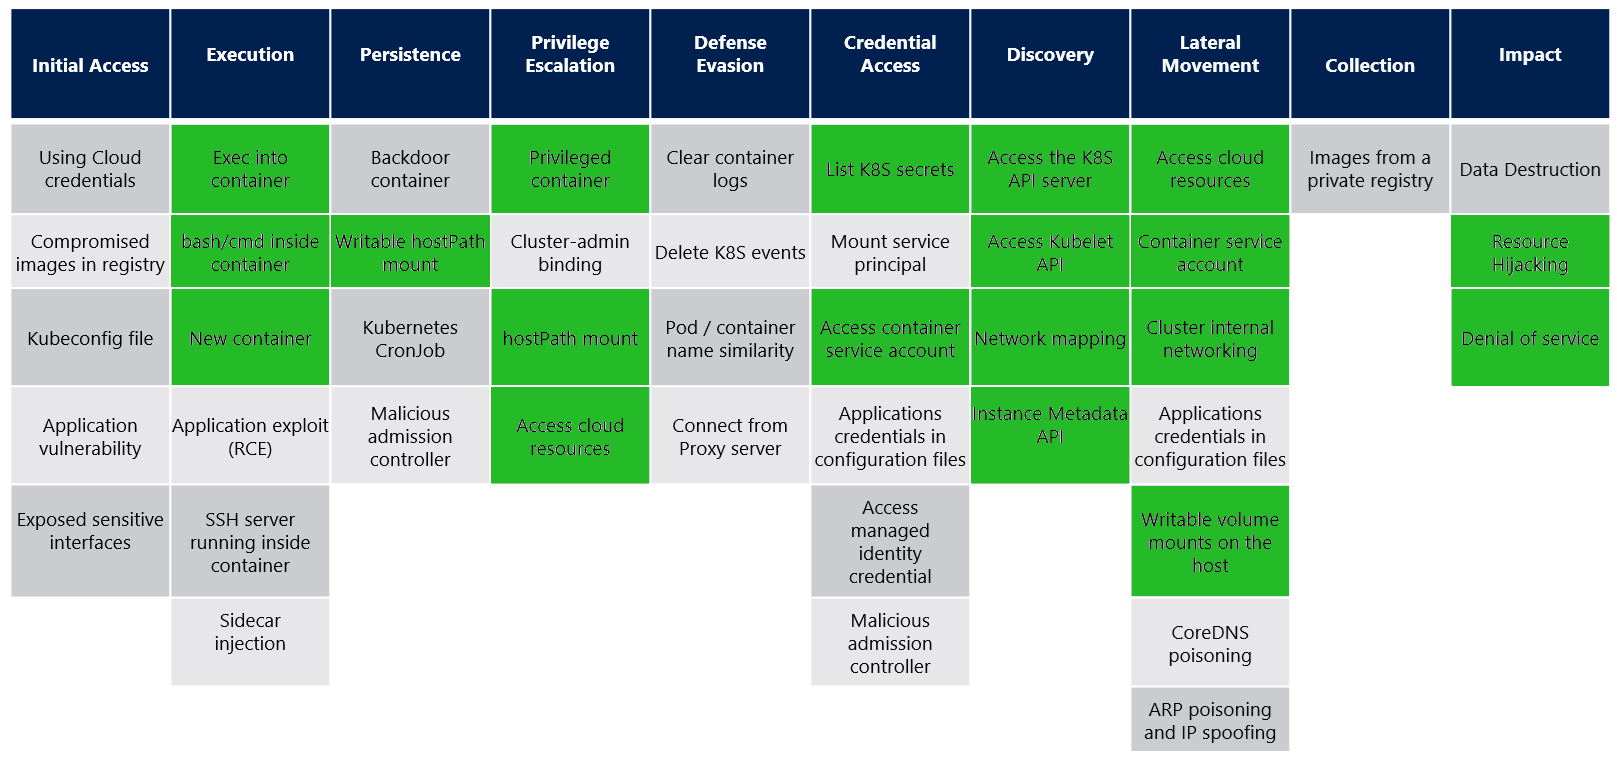
\includegraphics[width=\linewidth]{files/Matrix.png}
  \caption{Kubernetes threat matrix. The attack techniques addressed are highlighted in green.}
  \label{fig:threat-matrix}
\end{figure}

\subsection{Attacker model}

The adversary in this model is a compromised sidecar container in the cluster.
Since sidecar containers do not technically differ from main containers, they are compromised in a similar fashion.
For example, the cluster could run a container with security vulnerability or the admins could have been tricked into installing a malicious sidecar to the cluster.
Thus, the model assumes that the first stage is already breached.
The model also assumes that the adversary has execution capabilities in the sidecar container, specifically shell access to the sidecar container in the examples.
This type of security breach can occur if the application has a remote code execution (RCE) vulnerability that the attacker can exploit to run a reverse shell script inside the application.
As another example, the attacker could acquire valid credentials to an application running a Secure Shell (SSH) server through brute-force or phishing attacks.
The goal of the model is to prevent the attacker from escalating the attack from the initial breach.
Tables~\ref{table:threat-model} and \ref{table:threat-model-network} list the identified threats, with threats related to networking divided into the latter.

\begin{table}[H]
  \sffamily
  \centering

  \caption{Kubernetes sidecar threats}
  \label{table:threat-model}

  % minipage so that footnotes are printed
  \begin{minipage}{\textwidth}
  \renewcommand{\thempfootnote}{\arabic{mpfootnote}} % footnotes in minipage are letters instead of numbers, fixes that
  \begin{tabularx}{\textwidth}{CCC}
    \hline
    \textbf{Threat} & \textbf{Description} & \textbf{Mitigation} \\ \hline
    Privileged containers & If containers are given privileges, malicious actors can break out from the container and escalate the attack on the cluster. & Use \lstinline{restricted} Pod Security Admission to enforce security rules. PSAs are defined for namespaces, so isolate privileged containers into their own namespaces to follow the principle of least privilege. \\ \hline
    Writing to the host file system & If allowed, malicious actors can try to tamper with the application or write executables to a disk. & Do not allow unnecessary mounts. Use \lstinline{readOnlyRootFilesystem: true} whenever possible. \\ \hline
    Permissive RBAC on ServiceAccounts & Containers in a Pod share ServiceAccounts\footnote{\lstinline{spec.serviceAccountName} is a Pod-level field}. By default, Pods automatically mount the ServiceAccount to all containers. & Disable automatic mounting of ServiceAccounts\footnote{Set \lstinline{automountServiceAccountToken: false}} and explicitly mount them to containers when needed. Adhere to the principle of least privilege. \\ \hline
    There are no resource limits for containers & If not set, a single container can hog system resources, causing denial of service (DoS). & Set resource limits to containers\footnote{Use \lstinline{spec.containers[*].resources}}. \\ \hline
  \end{tabularx}
  \end{minipage}
\end{table}

\begin{table}[H]
  \sffamily
  \centering

  \caption{Networking threats for sidecars}
  \label{table:threat-model-network}

  \begin{minipage}{\textwidth}
  \renewcommand{\thempfootnote}{\arabic{mpfootnote}}
  \begin{tabularx}{\textwidth}{CCC}
    \hline
    \textbf{Threat} & \textbf{Description} & \textbf{Mitigation} \\ \hline
    The Pod has network access to the control plane & By default, all traffic inside the cluster is allowed. & Use NetworkPolicies as a firewall. Deny by default and explicitly allow traffic only if needed. \\ \hline
    Sidecar can use the main container's NetworkPolicy to access \emph{kube-system} or other Pods & NetworkPolicies affect the NIC of the Pod network, which is shared by sidecars. & \textbf{No built-in solution available!} \\ \hline
    Sidecar has network access to the main container & Main container is accessible via loopback device, which cannot be protected with NetworkPolicy. & \textbf{There is no built-in solution available!} \\ \hline
    Sidecar sniffs the main application traffic & Pod-to-Pod traffic in a cluster is unencrypted by default. A privileged sidecar can sniff and hijack traffic. & CNIs and service meshes may provide encryption to inter-Pod traffic with, for example, IPSec, Wireguard, and mutual TLS. These are often implemented with sidecars, which is not feasible in this scenario. For intra-Pod traffic, containers would need to implement this as part of the containers. \\ \hline
  \end{tabularx}
\end{minipage}
\end{table}

One of the worst-case scenarios is that the attacker has access to a privileged sidecar container.
A privileged container has all the capabilities of the host machine, so basically a root user inside a privileged container means that the attacker has root privileges on the host Node.
Furthermore, the container lacks restrictions from Seccomp, AppArmor, and Linux capabilities.
The Listing~\ref{lst:privileged-container} describes a Deployment with a privileged container with extremely insecure specifications.

\lstinputlisting[
  caption={Privileged container},
  label={lst:privileged-container},
  language={yaml}
]{code/privileged.yml}

The three first fields in the \lstinline{spec} remove namespace isolations from the container and use the corresponding Node namespaces instead.
With a privileged container and \lstinline{hostPID: true}, the attacker can enter Node's namespace with \lstinline{nsenter} (easy target PID is the \textbf{init} system running as 1), and execute commands on the host.
The attacker can also see and enter other containers and processes running on the same Node.
In a non-privileged container, \lstinline{hostPID} still allows Denial of Service (DoS) attacks by killing the processes on the Node.

Since the container mounts the host filesystem to a volume in \lstinline{/host-root}, the attacker in a privileged container can trivially use \lstinline{chroot} to execute commands as the root user in the host Node context.
Even without the explicit \lstinline{hostPath} mount, the host machine's \lstinline{/dev} is accessible from the privileged container, which means that the container can see the disk that contains the host's filesystem and mount the disk.
The attacker can use this technique to find any credentials stored on the host machine and escalate the attack.
Important credentials include, for example, \lstinline{kubeconfig} files that store access tokens to the Kubernetes API server, ServiceAccount tokens that may have been mounted on any Pod on the host, SSH keys and hashed user passwords in \lstinline{/etc/shadows}.

The biggest risks considering a non-privileged container with all the isolations intact relate to lateral movement and the discovery of secrets.
Kubernetes automatically mounts each container in a Pod with a ServiceAccount token, which can be used to attack the control plane if it is over-permissive.
Since the cluster has no NetworkPolicies in place by default, any misconfigured control plane component, such as Kubelet or API server with \lstinline{anonymous-auth} set to true, could be exploited.
In addition, the attacker can try to breach or DoS any control plane component or workload in the cluster, or other connected services like those in a cloud-hosted system.
Furthermore, any unpatched vulnerability in the underlying kernel, container runtime, or Kubernetes can exploited.

The \emph{malicious-sidecar} image is a simple custom-made container image that includes some basic tools for penetration testing.
The image also installs \lstinline{kubectl} and sets environment variables so that the CLI tool works out of the box with the default Minikube installation.
Its Dockerfile can be found in Appendix~\ref{app:malicious-sidecar}.
If the container has public Internet access, the attacker could use a tool such as Docker Enumeration, Escalation of Privileges, and Container Escapes (DEEPCE) \cite{deepce} to enumerate attack options even further.

\clearpage

\section{Solution requirements} \label{sec:methods}

This chapter defines the security requirements of the solutions that are discussed in the following chapters. This chapter also introduces the development environment which is used to test and implement the solutions.

\subsection{Security requirements}

Threat modeling identified two main categories of issues: permissive workload configurations and networking-related issues.
Essentially, all threats are caused by sidecars not respecting the principle of least privilege; the sidecar inherits execution and networking privileges from the main application container.
Based on the model, the solution should provide answers to these main questions:

\begin{enumerate}
  \item How to ensure and enforce that workloads that conflict with the principle of least privilege are not deployed to the cluster?
  \item How to enforce Zero Trust network that allows traffic filtering on the container-level and limits communication on both loopback and Pod network interface devices?
\end{enumerate}

Regarding the first question, the existing mitigations were already listed in Table~\ref{table:threat-model} while threat modeling.
A solution in which all mitigations are applied is introduced in Chapter~\ref{sec:pod-hardening}.
For the second question on building the Zero Trust network, the Pod must be firewalled for both inter-Pod communications on the Pod network NIC and intra-Pod communications on the loopback NIC.
However, Kubernetes does not provide any built-in solution for creating these firewalls.
A few possible solutions for building the Zero Trust network inside the Pod are given in Chapter~\ref{sec:network-solution}.

\subsection{Environment}

The solution is tested and developed on a Minikube v1.32.0 cluster running on a local machine and using Docker as the driver for Nodes.
The cluster consists of two Nodes, the purpose of which is to deploy control plane components separately from worker ones.
Furthermore, the setup also allows testing of network between components hosted on different Nodes.
The complete setup is hosted on GitHub (https://github.com/Arskah/k8s-sidecar-security).
Both Calico and Cilium are used as CNI plugins since the selection of CNI plugins has minor implications on the actual networking solution. %TODO:
The implications are discussed in detail in Chapter~\ref{sec:network-solution}.

A simple Node.js webserver with a StatsD metrics aggregation sidecar is used as the application workload.
The source code for the webserver can be found in Appendix~\ref{app:node-webapp}, while a StatsD debugging container called \lstinline{hypnza/statsd_dumpmessages} is downloaded from Dockerhub \cite{statsd-container}.
The webserver serves "Hello world" on port \lstinline{8888} and sends response times and other metrics as UDP messages to the StatsD sidecar on default port \lstinline{localhost:8125}.
The sidecar prints incoming stats verbosely to stdout.

For penetration testing purposes, another sidecar is introduced with common networking and Kubernetes command line tools.
When deployed instead of the StatsD client, this sidecar can be used to simulate situations where the attacker has managed to get access to the shell inside the sidecar.
The Dockerfile for the image can be found in Appendix~\ref{app:malicious-sidecar}.

\clearpage

\section{Hardening Pod security} \label{sec:pod-hardening}

This chapter provides a solution for hardening Pods against privilege escalation attacks.
The solution enforces that deployed resources follow Kubernetes' best security practices.
Most of the practices are enforced by the built-in Pod Security Admission controller.
However, this chapter also introduces additional security measures that fix a few oversights regarding sidecar containers in the controller.

\subsection{Restricted Pod Security Standard}

Since version 1.25, Kubernetes has shipped with the Pod Security Admission controller as a stable feature.
The controller, as discussed in Chapter~\ref{admission-controllers}, provides three different Pod Security Standards that can be used to warn and enforce against insecure Pod configurations.
The \lstinline{restricted} Pod Security Standard is the strictest of the standards and aims at the best Pod hardening practices \cite{k8s-docs-pss}, so it will be the most optimal for our solution.
The Security Standard can be easily enforced by adding \lstinline{pod-security.kubernetes.io/enforce: restricted} as a label on a Kubernetes namespace resource, as shown in Listing~\ref{lst:pss}.

\lstinputlisting[
  caption={Namespace resource with \lstinline{restricted} Security Standard},
  label={lst:pss},
  language=yaml
]{code/restricted-ns.yml}

Table~\ref{table:pod-hardening} illustrates the fields that the restricted security standard affects.
From the table, it can be noted that the standard already blocks 2 out of the 4 identified threats: the deployment of privileged containers and host directory mounts.
However, it should be noted that the standard restricts the networking solution discussed in the following chapter.
Since the security standard only allows for the \lstinline{NET_BIND_SERVICE} capability, any Pod attempting to modify the network stack will not work.
Therefore, network modifications must be implemented outside of the Pod's context, which is discussed in greater detail in Section \ref{sec:network-solution:deployment}.

\begin{table}[H]
  \centering
  \caption{Pod fields enforced by \lstinline{restricted} Security Standard}
  \label{table:pod-hardening}
  \sffamily
  \small
  \begin{minipage}{\textwidth}
  \renewcommand{\thempfootnote}{\arabic{mpfootnote}}
  \begin{tabularx}{\textwidth}{CCC}
    \hline
    \textbf{Field name} & \textbf{Usage} & \textbf{Allowed values}\\ \hline
    \lstinline{hostPID}, \lstinline{hostIPC}, \lstinline{hostNetwork} & Controls whether the container uses the host's PID, IPC, and network namespace. & \lstinline{false} \\ \hline
    \lstinline{privileged} & Controls whether Pod can run privileged containers. & \lstinline{false} \\ \hline
    \lstinline{capabilities.add} / \lstinline{drop} & Defines Linux capabilities for the container. & Add \lstinline{NET_BIND_SERVICE} allowed, drop \lstinline{ALL} required \\ \hline
    \lstinline{volumes[*]} & All volume types are not allowed. For example, hostPath, which maps host directories, is not allowed. & \lstinline{configMap}, \lstinline{csi}, \lstinline{downwardAPI}, \lstinline{emptyDir}, \lstinline{ephemeral}, \lstinline{persistentVolumeClaim}, \lstinline{projected}, \lstinline{secret} \\ \hline
    \lstinline{hostPort} & Expose the container via the host's network port. & Must not be defined \\ \hline
    AppArmor annotation\footnote{\lstinline{container.apparmor.security.beta.kubernetes.io/*}} & Sets the AppArmor profile used by containers. & \lstinline{runtime/default}, \lstinline{localhost/*} \\ \hline
    \lstinline{seLinuxOptions} & Sets the SELinux context of the container. & Set if supported by the environment. \\ \hline
    \lstinline{procMount} & The default \lstinline{/proc} masks are set up to reduce the attack surface. & \lstinline{Default} \\ \hline
    \lstinline{seccompProfile.type} & Sets the Seccomp profile used to sandbox containers. & \lstinline{RuntimeDefault} or \lstinline{Localhost} \\ \hline
    \lstinline{sysctls[*].name} & Sysctls can disable security mechanisms or affect all containers on a host. &  and All disallowed except for an allowed "safe" subset \footnote{\lstinline{kernel.shm_rmid_forced, net.ipv4.ip_local_port_range, net.ipv4.ip_unprivileged_port_start, net.ipv4.tcp_syncookies, net.ipv4.ping_group_range}} \\ \hline
    \lstinline{allowPrivilegeEscalation} & Controls whether the process can gain more privileges than the parent. & \lstinline{false} \\ \hline
    \lstinline{runAsNonRoot} & Controls whether the container can run as the root user. & \lstinline{true} \\ \hline
    \lstinline{runAsUser}, \lstinline{runAsGroup} & Controls the user and group used by the container. & Set both to non-zero to run as non-root. \\ \hline
    \lstinline{windowsOptions.hostProcess} & Runs Windows containers as privileged HostProcess. & \lstinline{false} \\ \hline
  \end{tabularx}
  \end{minipage}
\end{table}

\subsection{Enforcing other best practices}

The \lstinline{restricted} Security Standard hardens the Pod against most of the identified security threats.
However, it still does not enforce specific resource limits and allows automatic mounting of ServiceAccounts for the Pod containers.

Adding resource limits to containers is straightforward: just add values to both \lstinline{resources.limits.cpu} and \lstinline{resources.limits.memory} fields for all of the containers, similar to the Listing~\ref{lst:service-account-mount}.
The CPU usage is measured in CPU units and can also be expressed in millicpus, i.e., both an integer value of 1 and "1000m" are equivalent to 1 physical or virtual core \cite{k8s-docs-resources}.
For memory, the base unit is bytes, but it also supports quantity suffixes such as "M", "Mi", and "Gi" for megabytes, mebibytes, and gigibytes, respectively.
The resource limits are registered to the container's cgroups by the Kubelet.
Limits are hard, which means that if a container exceeds its CPU limit, execution is blocked until more CPU capacity is available.
Exceeding the memory limit causes termination with an out-of-memory (OOM) error.

\subsubsection{Manual ServiceAccount mounting}

By default, the ServiceAccount tokens are mounted in the \lstinline{/var/run/secrets/kubernetes.io/serviceaccount} directory in every container.
This feature can be disabled by setting \lstinline{automountServiceAccountToken: false}, but then any container that actually uses the ServiceAccount must receive the token in some other way.
Since volume mounts are defined per container and ServiceAccount tokens can be created manually with Secrets, the issue can be circumvented by manually mounting the token to containers that use it.

\lstinputlisting[
  caption={ServiceAccount with permissions for fetching Pod resources},
  label={lst:service-account},
  language={yaml}
]{code/SA.yml}

Listing~\ref{lst:service-account} shows how to create a ServiceAccount token with permission to read the status of Pods in the cluster.
While Role, RoleBinding, and ServiceAccount resources are used to create and define RBAC rules for the ServiceAccount, the Secret resource creates a similar authorization token as Pod with auto-mounting of ServiceAccount tokens would create and mount on the containers.
When the token created by the Secret resource is mounted to the same path as the automatic mounting, as in Listing~\ref{lst:service-account-mount}, the token is only mounted to the container that needs it.
With this approach, the account tokens are only mounted into containers that actually need them, and the tokens cannot be used for privilege escalation from other containers of the Pod.

\lstinputlisting[
  caption={Two container Pod with resource limits and manually mounted ServiceAccount},
  label={lst:service-account-mount},
  language={yaml}
]{code/SA-mounted.yml}

\subsubsection{Enforcing the fields}

Kubernetes' Admission controller is the go-to tool for preventing undesired configurations from entering the cluster.
Unfortunately, the existing built-in hooks do not provide the option to enforce resource limits or manual ServiceAccount mounting.
As there is no existing community solution, a custom-made ValidatingAdmissionWebhook needs to be created.

The GitHub development setup includes an example admission controller based on Slack's \emph{simple-kubernetes-webhook} \cite{simple-kubernetes-webhook}.
A template is supplemented with a custom validation function, \emph{resource-validator}, which is shown in Listing~\ref{lst:resource-validator}.
When a Pod specification with no \lstinline{resource.limits} definition is validated, the if-statement on line 20 triggers, causing the validation to fail.
The function can be trivially extended to allow CPU and memory values only in a given range.

\lstinputlisting[
  caption={Go function for validating that resource limits are used},
  label={lst:resource-validator},
  language={Golang}
]{code/resourceValidator.go}

The validator for automatic mounting of ServiceAccounts could be implemented similarly.
Instead of verifying resource limits, the function should verify that \lstinline{PodSpec.AutomountServiceAccountToken} is set to false.

Custom Admission controller webhooks require a Deployment and a Service resource, as well as TLS certificates stored as a Secret resource.
These resources are well-documented in the \emph{simple-kubernetes-webhook} example.
The example also provides a shell script for minting TLS certificates.
However, in production environments, the TLS certificates should be generated by a specialized certificate manager workload installed in the cluster.
Because of the effort needed to include production-ready webhooks in the demonstration setup, these are left as an exercise for the reader.

\clearpage

\section{Network Isolation} \label{sec:network-solution}

Implementing a zero-trust network architecture in a Kubernetes cluster is not trivial, since building network isolation between containers in the same Pod is not possible with common CNI plugins and NetworkPolicies.
The root cause for this is that the lowest level of networking abstraction in Kubernetes is the Pod and that by definition all containers in a Pod share network namespace.
Thus, all traffic outside the Pod, from any of the containers, passes through the same \emph{eth0} NIC and shares a common source IP address.
Since NetworkPolicies operate on L3/L4, they cannot distinguish whether traffic originates from the sidecar or from the main container.
Although the ingress traffic can be easily identified with the destination port number, the source port for the egress traffic depends on the TCP implementation.
As a result, NetworkPolicies cannot be used to manage egress traffic from the sidecar independently of the main container.
For intra-Pod communication, traffic passes through the loopback device, which is created by a \emph{loopback} plugin \cite{k8s-docs-cni}.
The plugin is not managed by the CNI plugin installed on the Nodes; instead, Kubernetes requires that the underlying container runtime provides the implementation.
Most runtimes implement the reference CNI plugin \cite{cni-loopback}, but, for example, CRI-O implements its own.
Due to this, the plugin does not install with a controller that would enforce NetworkPolicies on the loopback device.
Furthermore, since all intra-Pod traffic has source and destination IP addresses of \lstinline{127.0.0.1}, the packets do not have clear identifiers that could be used for traffic filtering.
This chapter introduces two general approaches to solving the issue.

The first solution enforces firewall rules inside the application Pod's network namespace, while the second approach creates network namespaces for each container by deploying them to their own Pods.
While deploying containers in their own Pods is an obvious option for creating isolation, the approach breaks the tight integration of sidecar containers to the application container.
Most importantly, sidecars will have their own independent lifecycle and scheduling, and communication via the loopback device will be broken.
In the scope of this thesis, we consider sidecars to be scheduled along the application container and accessible via \lstinline{127.0.0.1}.
Thus, re-introducing these characteristics to the containers is also part of the solution.

\subsection{Applying firewall rules inside Pod network namespace}

\begin{figure}[h!]
  \centering
  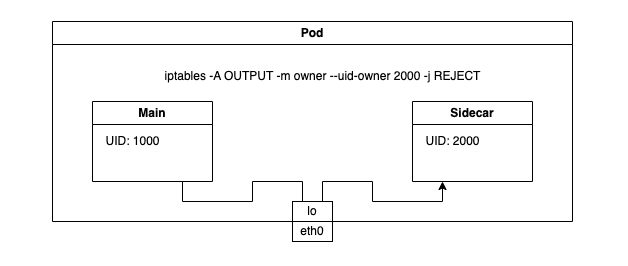
\includegraphics[width=\linewidth]{files/iptables.png}
  \caption{Single network namespace architecture}
  \label{fig:single-net-solution}
\end{figure}

Figure~\ref{fig:single-net-solution} illustrates the network architecture with all required network rule enforcement points.
The solution needs to enforce network rules in four scenarios: i) external components and Pod's \emph{eth0}, ii) main container and \emph{lo}, iii) sidecar container and \emph{lo}, and sidecar container and \emph{eth0}.
The ingress and egress rules in the first scenario are more easily enforced with \textbf{NetworkPolicies}, as shown in Listing~\ref{lst:network-policy}.
The policies allow cluster and external traffic to the main application port \lstinline{8888} while denying all other traffic to and from the Pod.

\lstinputlisting[
  caption={NetworkPolicy handling traffic between Pod and external components},
  label={lst:network-policy},
  language={yaml}
]{code/zero-trust-policy.yml}

The other scenarios cannot be enforced with NetworkPolicies, since the rules depend on individual containers instead of Pods.
The rules need to be applied inside the Pod's network namespace with tools such as IPTables.

\subsubsection{IPTables}

% https://www.frozentux.net/iptables-tutorial/iptables-tutorial.html#OWNERMATCH
Usually, IPTables rules are applied to packets by their IP addresses and ports.
However, modern versions of IPTables ship with an owner module, which supports rules based on the process's name and user, group, process, and session identifiers \cite{iptables-manpage}.
For example, \lstinline{iptables -A OUTPUT -m owner --uid-owner 1000 -j REJECT} would reject all egress packets from containers with the specific user ID.
While the session identifier is assigned at runtime by the kernel, containers' user and group IDs can be overridden with Pod definition's \lstinline{runAsUser} and \lstinline{runAsGroup} fields, respectively.
Thus, any ingress or egress traffic of a container with a unique user identifier can be filtered with IPTables.

Listing~\ref{lst:iptables-bash} shows IPTables rules that can enforce network rules in other scenarios.
As ingress rules, the main application port is opened on all network devices, while the sidecar port is only allowed on the loopback device.
For egress traffic, the main application is given access to both containers' ports, while the sidecar can only access its own port.
All other traffic is rejected by default.

\lstinputlisting[
  caption={IPTables rules for the Pod},
  label={lst:iptables-bash},
  language={bash}
]{code/iptables.sh}

The approach is similar to how Istio redirects all Pod traffic through the Envoy sidecar and the service mesh.
Istio adds IPTables rules that reroute all traffic, except those originating from user id 1337, to the Envoy proxy \cite{istio-iptables}.
The user ID itself is reserved for the proxy, and it is used to avoid re-routing the proxy traffic, which would cause an infinite loop.

eBPF programs were also considered as an option for IPTables.
Since XDP programs support only ingress rules, they are not a valid option for solving the problem.
However, a traffic control (TC) program that could distinguish sidecar container traffic from others could be a possible option.
TC programs manipulate packets by modifying \lstinline{struct __sk_buff} in the user space.
The complete C structure is listed as Listing~\ref{lst:sk-buff}.

\lstinputlisting[
  caption={\lstinline{skbuff} struct in Linux v6.3 \cite{linux-kernel-skbuff}},
  label={lst:sk-buff},
  language={C}
]{code/skbuff.c}

As can be seen in the example, the structure has no identifiers that are unique for each container.
A notable attribute in the structure is the \lstinline{mark} field, which can be used as an identifier for the packet in the kernel.
It does not propagate with the packet, which means that marking can only be used for traffic filtering before the packet leaves the network stack.
When combined with an IPTables rule that uniquely marks the packets egressing from the sidecar, for example, setting the mark as 2 \lstinline{iptables -t mangle -A PREROUTING -m owner --uid-owner 1000 -j MARK --set-mark 2}, a TC eBPF program could be used to filter traffic.

However, using eBPF brings an extra layer of complexity in comparison to simply using IPtables for traffic filtering.
Furthermore, eBPF programs do not provide any performance gains for egressing traffic, since the TC hooks execute after the packet has been processed by IPTables.
Due to the above reasons, the solution relies only on IPTables rules for packet filtering.

\subsubsection{Deployment} \label{sec:network-solution:deployment}

The commands for creating the IPTables rules could be applied to the Pod with an initContainer or postStart lifecycle handler.
However, the commands require root user permissions with \lstinline{NET_ADMIN} and \lstinline{NET_RAW} capabilities and would require changing Pod's security admission level to privileged.
Thus, it is more optimal to apply the rules outside the Pod context and Namespace; for example, by using a controller in an operator pattern.
The same capabilities are paramount to any CNI plugin controllers that enforce NetworkPolicies using IPTables or eBPF.

For demonstration purposes, a custom container is used and installed with IPTables and \lstinline{crictl} CLI.
The container uses \lstinline{crictl} to find the PID of a container in the Pod and uses \lstinline{nsenter} to apply the IPTables rules inside the container's network namespace.
The Dockerfile is found in Appendix~\ref{app:iptables-injector}, and the DaemonSet is shown in the following Listing~\ref{lst:iptables-injector}.

\lstinputlisting[
  caption={DaemonSet for a container injecting IPTables rules inside Pods},
  label={lst:iptables-injector},
  language={yaml}
]{code/iptables-injector.yml}

The script is not a valid controller as it does not implement a control loop that reacts to Pod creation.
Instead, it only works when it is executed after the Pod has been created.
Therefore, it is only useful for demonstrating the concept and should not be used for purposes other than testing.
Additionally, DaemonSet requires extensive privileges: the \lstinline{crictl} that is used to find the PID must be run on a privileged Pod, and the \lstinline{nsenter} command needs access to the host PID namespace.

\subsection{Own network namespace for sidecar}

\begin{figure}[h!]
  \centering
  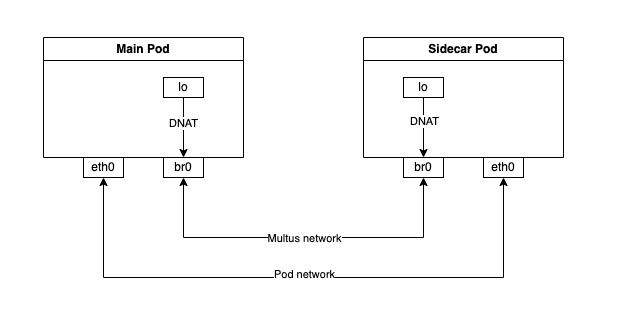
\includegraphics[width=\linewidth]{files/multus.png}
  \caption{Multiple network namespaces architecture}
  \label{fig:multi-pod-net-solution}
\end{figure}

The network architecture for the solution, where containers are deployed in separate Pods, is shown in Figure~\ref{fig:multi-pod-net-solution}.
The idea behind this approach is to utilize custom resources to regulate traffic between the containers, similar to NetworkPolicies.
As containers are no longer considered sidecars, the solution must establish communication using the \lstinline{localhost} address.

Although it is possible to use the default network created by the CNI plugin for sidecar traffic, the proposed solution creates a new isolated network for traffic with Multus.
The isolation allows the use of a separate IP address pool for the traffic, simplifying the re-implementation of loopback communication with a straightforward redirection rule.

\subsubsection{Creating an isolated network for sidecar traffic}

It is completely possible to use the default Pod network created by the CNI plugin for traffic between sidecars.
With this setup, the network rules are simply NetworkPolicies on top of the policy that implicitly denies all other traffic.

It is also possible to build new network interfaces for sidecar traffic with Multus.

\lstinputlisting[
  caption={NetworkAttachmentDefinition for creating MacVLAN bridge between the Pods},
  label={lst:attachment},
  language={yaml}
]{code/attachment.yml}

The setup requires creating \textbf{NetworkAttachmentDefinition} CRD for the network.
Each Pod that should be part of the network needs a \lstinline{k8s.v1.cni.cncf.io/networks} annotation, as seen in Listing~\ref{lst:pod-with-bridge}.

\lstinputlisting[
  caption={Deployment with Pod connected to the bridge},
  label={lst:pod-with-bridge},
  language={yaml}
]{code/minimal-deployment.yml}

The common NetworkPolicies are not applied to the Multus network.
However, the Multus developers have introduced another CRD, \textbf{MultiNetworkPolicy} \cite{multi-network-policy}, which mimics NetworkPolicies but only works for networks created by Multus.
The resource is identical to NetworkPolicies, as seen in the Listing~\ref{lst:policies}.

\lstinputlisting[
  caption={Zero trust MultiNetworkPolicies for br0 network interface},
  label={lst:policies},
  language={yaml}
]{code/multi-network-policies.yml}

However, the Multus CNI does not enforce the \textbf{MultiNetworkPolicy} rules in any way.
The implementation is left for other DaemonSets such as \emph{multi-networkpolicy-iptables} \cite{multi-network-policy-iptables} and \emph{multi-networkpolicy-tc} \cite{multi-network-policy-tc}, both of which are created by the Multus team.
As the names suggest, DaemonSets implement the enforcement with IPTables and eBPF TC programs, respectively.
The \emph{multi-networkpolicy-iptables} is used for the solution since IPTables implements all other network rules for the cluster.

% TODO: Check the security of this https://github.com/kubernetes/kubernetes/issues/90259
% https://security.stackexchange.com/questions/137602/what-are-the-security-implications-of-net-ipv4-conf-eth0-route-localnet-1-rout

With these configurations and dependencies, the containers should have a new network and reach each other via the bridge interface.
As the next step, the solution must find a way to redirect traffic destined for the localhost to the new network.
The script in Listing~\ref{lst:dnat} shows how to redirect all egressing traffic with IPTables from the source of \lstinline{127.0.0.1:8125} to another network interface with an external IP address, like \lstinline{192.168.1.202:8125}.
By default, the re-routing of local traffic outside the local machine is denied by the kernel.
To overrule this default behavior, the script sets a kernel flag with \lstinline{net.ipv4.conf.all.route_localnet=1}.

\lstinputlisting[
  caption={Script for mapping localhost to br0 interface},
  label={lst:dnat},
  language={bash}
]{code/localhost.sh}

The demo solution on GitHub uses the same \emph{iptables-injector} daemon container introduced in \ref{sec:network-solution:deployment} for running the above script in container namespaces.

\subsubsection{Co-scheduling the containers}

The configuration described above does not replicate the behavior of traditional sidecars.
The sidecar is specified in a separate Deployment resource, meaning it has a distinct lifecycle from the main container.

MutatingAdmissionWebhooks can be used to modify the Pod \emph{CREATE} and \emph{DELETE} actions so that the sidecar Pod is created and deleted in tandem with the main container.
However, MutatingAdmissionWebhooks are designed only to operate on the resources sent to them.
Kubernetes documentation states that any webhook that makes out-of-band changes or has any other side effects should be accompanied by a controller that periodically determines the actual state of the cluster \cite{k8s-docs-dac}.

A custom controller watching for a specific sidecar annotation could also implement co-scheduling; however, the controller must somehow keep track of which Pod the sidecars are assigned to.
With this information, the controller could react to Pod lifecycle events, and fully support scaling, restarting, and cleanup of sidecar containers.
Because of the complexity and the amount of work required to implement co-scheduling, this feature has been left out of the solution and is something to consider in the future.

\clearpage

\section{Solution Evaluation} \label{sec:solution}

This chapter demonstrates with experiments that the solutions presented in Chapters \ref{sec:pod-hardening} and \ref{sec:network-solution} effectively isolate containers within the same Pod from one another.
The evaluation not only verifies that the solutions meet the requirements but also examines their potential and any weaknesses that can be improved.

The experiments in the first section involve assessing security admission by deploying privileged Pods to the cluster, as well as enforcing network isolation by generating intra-Pod and inter-Pod HTTP traffic with client tools such as \lstinline{curl}, \lstinline{wget}, \lstinline{kubectl} and \lstinline{netcat}.
The \emph{malicious-sidecar} container (outlined in Appendix \ref{app:malicious-sidecar}) is added to the application containers as an additional sidecar and serves as an entry point for attacks in the experiments.
The container has all the necessary tools installed.

\lstinputlisting[
  language={yaml},
  label={lst:attacker},
  caption={Configuration of the third, malicious container added to the deployments}
]{code/attacker.yml}

Both network isolation solutions should only permit UDP traffic from the webserver container to the StatsD client.
Any other successful request is deemed a failure in isolation.
The second section examines the qualitative characteristics of the solutions, such as any observed limitations in security or usability when the solutions are used in production environments.

\subsection{Security Evaluation}

The experiments in this section verify that network isolation works correctly in both solutions.
As a prerequisite for the experiments, the built-in Pod Security Admission rules should be enabled for the environments.
To verify this, the first step in the evaluation is to deploy a Pod that is overly permissive into the cluster.
The Deployment used to test this is shown in Listing~\ref{lst:privileged-container}.
The definition namespace metadata fields were altered to match the namespace being tested, for example, \lstinline{app} in our case.

When trying to deploy the Pod to the test cluster, a warning (illustrated in Listing~\ref{lst:psa-warning}) is displayed, which prevents deployment.
This shows that Pod Security Admissions is functioning properly in the test environment, confirming the prerequisite, and allowing the evaluation to progress to testing network isolation.

\lstinputlisting[
  language={bash},
  label={lst:psa-warning},
  caption={Warnings printed to terminal by Pod Security Admission}
]{code/psa-warning.sh}

Experiments were conducted for both proposed solutions.
The first solution, which uses a single network namespace, was tested with both Docker and containerd runtimes.
However, since \emph{multi-network-policy-iptables} does not work with Docker, the Multus solution was only evaluated with containerd runtime.

\subsubsection{Experiment 1: sidecars cannot access main application}

The first experiment tests the main application's network isolation from sidecar threats.
As none of the sidecars in the system requires access to the main application container, isolation should block all requests from the sidecar containers.
This can be tested by sending an HTTP request from the attacking or StatsD sidecar to \lstinline{localhost:8888} with \emph{cURL}.
If isolation is successful, the request will be rejected.
This can be observed in the IPTables packet filter counters, which can be seen by using the \lstinline{iptables -xvn -L} command.

The first solution successfully rejected packets when it was used with Docker runtime.
However, when it was used with containerd, the packets were not rejected, even though the IPTables packet filter counters increased.
This suggests that there is a discrepancy in how the CRIs implement the loopback CNI, and that containerd's implementation might be optimized to bypass certain elements of the network stack.

The second solution also rejected the packets as expected.
Since it also implements the policies with IPTables, and containerd was used, this further implies that the unexpected result with the other solution is caused by how containerd implements the loopback CNI.

\subsubsection{Experiment 2: only main application can access StatsD sidecar}

The second experiment verifies that only the main application can send packets to the StatsD sidecar and that any other traffic directed there is blocked.
To test packet filtering rules, UDP packets are sent from the malicious sidecar to \lstinline{localhost:8125} with netcat (\lstinline{nc -u localhost 8125}).

The IPTables rules in the first solution reject the packets since the malicious-sidecar is deployed with a different user ID than the main application.
Similarly, the IPTables rules generated from MultiNetworkPolicies in the second solution filter the unwanted packets.

\subsubsection{Experiment 3: Access to other Pods is blocked}

The third experiment verifies that neither of the network solutions interferes with NetworkPolicies applied outside the Pod network.
The experiment environment uses a basic NetworkPolicy that blocks all outbound traffic and only allows inbound traffic to the main application.
Policies can be tested by trying to access, for example, \lstinline{google.com} or the Kubernetes API server from any container in the Pod.
From outside of the Pod, only the main application port should be reachable.

The two solutions both work as anticipated and do not conflict with CNI's NetworkPolicies.

\begin{table}[H]
  \sffamily
  \centering
  \caption{Experiment results}
  \label{table:evaluation-results}

  \begin{minipage}{\textwidth}
  \renewcommand{\thempfootnote}{\arabic{mpfootnote}}
  \begin{tabularx}{\textwidth}{CCCC}
    \textbf{Experiment} & \textbf{Solution 1, Docker} & \textbf{Solution 1, containerd} & \textbf{Solution 2, containerd} \\ \hline
    Isolated main & OK & Not OK! & OK \\ \hline
    Isolated sidecar & OK & Not OK! & OK \\ \hline
    Isolated Pod & OK & OK & OK \\ \hline
  \end{tabularx}
  \end{minipage}
\end{table}

\subsection{Qualitative assessment}

The above experiments verify that the proposed solutions can be used to implement the desired network isolation.
However, the solutions have several limitations and should only serve as a proof of concept.
These limitations should be mitigated before using the solutions in production environments.

The biggest limitation is that the solutions only function on specific container runtimes.
Since the first solution has only been proven to function on the Docker runtime, it logically limits the potential places where it can be used.
The limitation also raises the question of whether container runtimes should implement network isolation of sidecars.
Since the runtimes are responsible for creating the loopback device and they appear to have varying implementations of it, it may be impossible to create a tool at the orchestrator level that is not dependent on the runtime.

Additionally, \emph{multi-network-policy-iptables} does not function with Docker runtime.
The issue for this is vaguely documented in the project's GitHub issues \cite{multi-network-policy-iptables-bug}, but the issue was closed when Kubernetes dropped the explicit support for \emph{dockershim} in version 1.24.
Based on the experiments, the issue still exists on \emph{cri-dockerd} setups.
Furthermore, the documentation of \emph{multi-network-policy-iptables} explicitly states that it has not yet been released as a stable version.

From a security point of view, the primary drawbacks are associated with the IPTables policies and the injector daemon.
The first solution relies on distinguishing containers based on process user identifiers, which means that the system is only secure if the adversary cannot deploy containers with specific user IDs.
The current implementation does allow the adversary to deploy a container with an arbitrary user identifier, which means that an adversary with permission to create containers can bypass isolation.
Therefore, an admission controller is necessary to limit the allowed identifiers in production.

The injector daemon has the privileges to manage policies, so it should be regarded as a vital part of the cluster infrastructure, similar to CNI operators.
The current container has root privileges and access to the Node's container runtime socket, which could be exploited to compromise the entire Node.
To prevent this, the daemon's privileges should be reduced to the bare minimum.
CNI plugins with operators could be used as a model for this enhancement.
Furthermore, since the daemon does not function as a controller, the daemon needs to execute after application Pods are created to inject the IPTables rules.
As such, solutions cannot handle normal container lifecycle events.

In conclusion, the solutions are intricate and need to be further enhanced before they can be employed in the production environment.
The ideal solution would address the security issues mentioned above and implement a functioning controller loop to support container lifecycle events.

\clearpage

\section{Discussion \& conclusion} \label{sec:discussion}

\subsection{Future considerations}

This chapter examines potential improvements to the proposed solution.
As previously discussed, the proposed solution should not be used in production environments.
A production-ready solution should incorporate a valid controller loop instead of the shell script that was proposed.
Additionally, instead of relying on raw IPTables rules, the ideal solution should describe the policies with a custom resource, similar to NetworkPolicies.
The controller loop should be responsible for managing both Pods and policy resources, similar to how many CNI plugins have been designed to accommodate NetworkPolicies.
In contrast to common CNI plugins, the solution does not require the implementation of a CNI plugin, as the container runtime generates the loopback network interface.
However, it is important to ensure that the selected container runtime does not require connectivity via the loopback device, which would be blocked by the applied policies.

\subsection{Future of sidecars and service mesh}

The release of Kubernetes version 1.28 in August 2023 brought with it the new "SidecarContainers" feature gate.
This alpha-stage feature is designed to address the lifecycle and Pod termination issues that are currently experienced with sidecar containers \cite{k8s-v1-28-changelog}.
Although existing Kubernetes primitives are capable of adequately managing sidecars, they are not sufficient for certain use cases \cite{k8s-sidecar-kep}.
For example, service mesh sidecars must be running and ready before other containers to ensure that all traffic is routed through the mesh.
Similarly, if the sidecar terminates before other containers during shutdown, traffic from other applications may be lost.
Additionally, lifecycle-related issues can impede log- and metric-collecting sidecars, forcing applications to resort to unconventional workarounds.
Furthermore, in the event of an OOM error, the sidecar will not restart for jobs with \lstinline{restartPolicy: Never}.
This can render the application unreachable, as is the case with service meshes since the sidecar is necessary for application networking.

The introduction of sidecar containers as a new type of initContainer has made it easier to initiate and combine initContainers and sidecars in the start-up sequence.
However, the proposal explicitly states as a non-goal that it does not allow the enforcement of different security regulations for sidecars compared to other containers.
Therefore, it does not appear that the lowest security boundary will change from Pod to container in the near future.
Nevertheless, the new distinction between sidecars and other containers could allow this development in the future.

From a security standpoint, the safest option is to avoid sidecars altogether.
It is worth mentioning that the sidecar proxy is not a requirement for the implementation of a service mesh.
For example, Cilium service mesh uses eBPF for network layer operations and an Envoy proxy per host for application layer operations such as L7 load balancing and policies \cite{cilium-114}.
For sidecarless mTLS, Cilium combines TLS handshake and network-level encryption with IPSec or Wireguard.
This means that the service mesh can actually operate without a proxy in some cases, and the proxy container is only used when necessary.
The Envoy proxy is included in the cilium-operator, but since Cilium version 1.14, which was released in July 2023, the proxy can also be deployed as a DaemonSet independently.

Istio's service mesh also facilitates a sidecarless architecture.
Ambient mesh \cite{istio-ambient-mesh}, currently available as an open alpha version, uses ZTunnel proxies on each Node to provide L4 service mesh features such as mTLS, telemetry, authentication, and authorization.
However, the ZTunnel is not capable of handling any L7 features, which are instead implemented by a waypoint proxy.
The proxy operates on a per-namespace and per-service account basis, and it applies to all Pods in the same namespace by default.
Sidecarless traffic encryption is enabled through encrypted HBONE tunnels.

Despite the advantages of sidecarless service mesh, it comes with its own drawbacks.
Since all Pods on the Node use the same proxy, it can be subject to multi-tenancy issues such as the "noisy neighbor" anti-pattern, where one workload uses an excessive amount of resources and affects the performance of other workloads.
Furthermore, the single proxy is a single point of failure, and if it fails, all Pods on the Node become unreachable.
Additionally, the proxy is a more attractive target for attackers, as it can be used to impersonate any Pod on the Node.

The architecture of service meshes is a subject of much discussion in the industry, and the sidecarless design is not necessarily the next step in their development.
In fact, the first service mesh, Linkerd, used the per-host proxy model in its version 1, but due to operational, management, and security issues, version 2 was based on sidecars.

\subsection{Conclusion}

This thesis provided an overview of containers, Kubernetes networking, sidecar design pattern, and Zero Trust security architecture.
It identified the security risks associated with sidecar containers in Kubernetes and showed how an adversary could exploit them.
For issues that could not be resolved with existing tools, the thesis proposed two proof-of-concept solutions for creating network isolation between the application and sidecar containers.
Although following best practices in hardening Kubernetes clusters can help, the architecture of Pods in Kubernetes makes it difficult to isolate sidecars.
The first proposed solution implements network isolation within the Pod's network namespace using IPTables, while the second solution creates a network that mimics the shared network namespace of sidecars.
Solutions demonstrate that it is possible to isolate sidecars; however, the complexity and special infrastructure required to overcome this architectural limitation quickly outweigh the benefits.
From a security standpoint, tried and tested components are always preferable to custom infrastructure that requires maintenance.

\clearpage

%% Bibliography
\thesisbibliography
\printbibliography

\clearpage

%% Appendices

\thesisappendix

\section{Dockerfile for penetration testing} \label{app:malicious-sidecar}

\lstinputlisting[
  caption={Dockerfile for penetration testing},
  language={Docker}
]{code/appendix/pentest/Dockerfile}

\clearpage

\section{Example webserver deployed with StatsD sidecar} \label{app:node-webapp}

\lstinputlisting[
  caption={Node.js server (\lstinline{index.js})},
  language={javascript}
]{code/appendix/app/index.js}

\clearpage

\lstinputlisting[
  caption={\lstinline{package.json}},
  language={json}
]{code/appendix/app/package.json}

\lstinputlisting[
  caption={Dockerfile for the server},
  language={Docker}
]{code/appendix/app/Dockerfile}

\clearpage

\section{Dockerfile for penetration testing} \label{app:iptables-injector}

\lstinputlisting[
  caption={Dockerfile for injecting IPTables rules},
  language={Docker}
]{code/appendix/iptables-injector.Dockerfile}

\clearpage

\section{Webserver and StatsD deployed with Multus networking} \label{app:multus-sidecar}

\lstinputlisting[
  caption={Server's K8s deployment resource},
  language={yaml}
]{code/appendix/multus/node-app.yml}

\clearpage

\lstinputlisting[
  caption={StatsD container's K8s Deployment},
  language={yaml}
]{code/appendix/multus/statsD.yml}

\clearpage

\lstinputlisting[
  caption={Network interfaces and policies},
  language={yaml}
]{code/appendix/multus/interfaces.yml}

\end{document}
